\documentclass[oneside,11pt,a4paper,swedish]{scrbook}
\usepackage[utf8x]{inputenc}
\usepackage{babel}
\pagestyle{headings}
\setlength\parskip{\medskipamount}
\setlength\parindent{0pt}
\usepackage{graphicx}
\usepackage{ae}
\usepackage{aecompl}
\usepackage{amssymb}
\usepackage{amsmath}
\usepackage{comment}

\usepackage[T1]{fontenc}
%\usepackage{bookman}
\usepackage{multicol}
\usepackage{tikz}

\newcommand{\tavla}[1]{\reversemarginpar{ \rule[-10mm]{0.1mm}{#1cm}}}
\newcommand{\startex}[1]{\subsubsection{Exempel}\begin{quote}#1\end{quote}}
\newcommand{\startexn}[2]{\subsubsection{Exempel #1}\begin{quote}#2\end{quote}}

\newcommand{\ovning}[1]{\subparagraph{Övning: #1}}
\newcommand{\slutex}{\begin{flushright} \rule{1ex}{1ex} \end{flushright}}

\newcommand{\svarsrad}{\begin{flushright} \rule{14cm}{0.2mm} \end{flushright}}
\newcommand{\asm}[1]{\texttt{#1}}




\makeatother
\begin{document}

\title{Skalor och nomogram\\{}}
\author{Michael Josefsson}
\date{}
%\setcounter{chapter}{1}
\tableofcontents
\chapter{Introduktion}
Detta häfte har flera syften, bland annat

\begin{itemize}
\item Visa hur bra skalor ska konstrueras och hur de ser ut för lätt avläsning
\item Visa hur de kan användas i ingenjörsmässiga tillämpningar
\item Visa hur dubbelskalor och nomogram konstrueras
\end{itemize}

Häftet kan läsas enbart för skalornas skull, dubbelskalor och nomogram kan ses som intressanta utvidgningar.

\section{Skalor}
En skala är i det här fallet en gradering längs en axel. Vi träffar på och använder skalor hela tiden, det kan vara på linjaler, måttband, barometrar, kartor, voltmetrar, tankmätare i bilen, termometrar osv. Sålunda kan skalor användas för att mäta avstånd, volymer, fysikaliska storheter och annat. 

Även om analoga skalor numera ofta ersatts av digitala displayer på mätinstrument av olika slag har den traditionella skalan definitiva fördelar. En position på en skala ger till exempel ofta mer direkt och snabb information med tillräcklig information: Till exempel ger en vanlig analog klocka redan efter ett ögonkast en uppfattning om tiden. En snabb blick ger omedelbart ''kvart över två'' och ofta behövs inte högre noggrannhet. 

En analog skala ger också snabbt en uppfattning om en storhet ändras långsamt eller fort. Något som inte är lika tillgängligt med en digital display som måste ''bläddra klart'' innan värdet kan avläsas.\footnote{Här kan man också nämna att visad noggrannhet inte alltid överensstämmer med faktiska värden. En spänning kanske visas som ''1.697 V'' med millivoltsiffra men kanske egentligen är ''1.7 V'' när voltmeterns prestanda analyserats.}

En skalas syfte är att meddela betraktaren en storhet av något slag. En skala måste av detta skäl vara lättavläst. Man ska inte behöva fundera på vad skalan beskriver eller vilket siffervärde den förmedlar. För denna skull måste skalor utformas på ett sätt som är bekant för användaren. En skala med ovanliga beteckningar eller oväntat utseende är en dålig skala, den tar längre tid att läsa av. En skala ska inte vara i vägen för förståelsen.

I denna text förekommer lineära och icke-lineära skalor. De förra utgör grunden för hur en skala skall se ut med sin indelning av enheter, tjocka och tunnare streck osv. De senare ärver alla utseenden från sina lineära motsvarigheter men är oftast logaritmiska.

\section{Noggrannhet}

Den enklaste lineära skalan är den som återfinns på en linjal eller ett måttband. Den kan vara graderad i centimeter och millimeter eller meter och centimeter, mer sällan meter, centimeter \emph{och} millimeter. Ofta finns även markeringar för att underlätta läsandet, där en linjal har gärna halv-centimetrar inritade och  ett måttband kan ha olikfärgade fält för närliggande decimetrar osv.

Graderingen utförs med hänsyn till syfte och användning. En 30 cm lång linjal utförs med ofta med millimeterskala medan det vanligen är ointressant med millimetergradering på ett 50 m långt måttband. 

Det är intressant att notera att det överhuvudtaget ofta är helt onödigt med en mätnoggrannhet som överstiger storleksordningen en procent: En vanlig bordslinjal är ofta 30 cm och är indelad i millimeter ($1/300=0.3 \% $), även ett 50 m måttband med angivna centimeter är indelad i ($1/5000=0.0002 \% $).\footnote{Man kan fundera över hur mycket ett sådant måttband töjs vid användning: Töjs det 10 cm är detta $10/5000=0.002 \% $ dvs hela 10 gånger mer!}

Oavsett längd på skalan är mer än tre nivåer av märkning ovanligt. Det kan handla om

\begin{itemize}
\item Centimeter och  millimeter, eller
\item Meter, decimeter och centimeter, eller
\item Grader Celsius och tiondelar därav eller
\item Volt och  tiondels volt
\end{itemize}

\section{Mätnoggrannhet}

Det är i praktiken ovanligt att en mätt storhet har en dynamik överstigande 100:1 eller 1000:1. Man mäter till exempel spänningar i enstaka volt ner till hundradels volt ($1.42\,\textrm{V}$) eller 10-tals volt ner till tiondels volt ($18.7\,\textrm{V}$), 100-tals volt ner till enstaka volt ($204\,\textrm{V}$). Man anger inte spänningar som $1.421\,\textrm{V}$, $18.333\,\textrm{V}$ eller $204.984\,\textrm{V}$. 



Detta leder naturligt in på frågan \emph{Hur noggrant kan man mäta?} 
En vanlig multimeter har en noggrannhet på i storleksordningen en procent. Ofta varierar dessutom mätnoggrannheten både med vilket mätområde som använts och dessutom med det faktiskt avlästa värdet. 

\startex{Vilken noggrannhet kan man förvänta sig på mätområdet 2000 mV med en Digital Multimeter av typen Uni-T UT131D?}

Ur databladet kan man läsa att för detta mätområde gäller 
\begin{itemize}
\item Upplösning \emph{Resolution}: 1 mV
\item Noggrannhet \emph{Accuracy:} $\pm(0.5 \% + 2)$
\end{itemize}

Med störst utslag på detta område, mätvärde på 1.999 V, beräknas noggrannheten som $1.999 \cdot 0.005= 10\,\textrm{mV}$ plus 2 siffror i upplösning dvs sammantaget $10+2=12\,\textrm{mV}$. Procentuellt är noggrannheten alltså $\pm (12/2000)= \pm 0.6\,\%$.

Kompletterad med andra spänningar kan noggrannheten beräknas som 

\begin{center}
\begin{tabular}{c|r|c}

Mätvärde (V) & Noggrannhet ($\pm$mV)\footnote{Avrundat uppåt} & Noggrannhet ($\pm$\%) \\
&  & av mätvärde\\
\hline
 1.999  & $1999 \cdot 0.005= 10 +2=12$  & 0.6\\
 1.500 & $1500 \cdot 0.005= 8 +2=10$ & 0.7\\
 1.000 & $1000 \cdot 0.005= 5 +2=7$ & 0.7\\
 0.500 & $ 500 \cdot 0.005= 3 +2=5$ & 1.0\\
 0.010 & $  10 \cdot 0.005= 0 +2=2$ & 20\\
\end{tabular}
\end{center}

Man ser tydligt hur noggrannheten urartar vid låga spänningar\footnote{Upp till 100 mV dominerar $\pm$ '+2' dvs  avläst 15 mV kan vara faktisk spänning 12--17 mV.}. En slutsats är att anpassa mätområdet till mätvärdet så att så stor del som möjligt av mätområdet används och oavsett hur man gör är en mätnoggrannhet överstigande 1 \% svår att uppnå.

%Dyrare mätinstrument kan ha bättre noggrannhet men någon revolutionerande förändring 

\slutex

Verkligheten är normalt inte så beskaffad att man behöver hantera en stor dynamik i mätvärden. När angav du din längd i annat än meter och centimeter (''1.84 m'') eller enbart  centimeter (''165 cm'')? Aldrig är det ''1 792 mm''.

%Med skjutmått kan mätas 0.0 -- 150.0 mm, upplösning 0.1 mm med nonieskala. Noggrannhet $0.1\%$. 

%Mikrometer 0.00 -- 25.00 mm, upplösning 0.01 mm. Noggrannhet $0.04\%$.



\section{Räknesticka}

Skalor har varit centrala för att förenkla beräkningar i flera århundraden. Med miniräknarens intåg har det dagliga bruket av skalor dock blivit sällsynt vilket är synd då en vana vid skalor fortfarande behövs för att konstruera och läsa av diagram. 

Under en lång tid användes \emph{räknestickor} som den nedan för allehanda ingenjörsberäkningar. Den baserar sig till stor del på addition av logaritmiska skalor för att utföra multiplikation och division. Precisionen  på ''bröstficks''-räknestickan i figuren är minst två siffror. För ytterligare noggrannhet användes räknestickor med längre skala där ungefär 30 cm långa skalor var det vanliga. 




\begin{center}
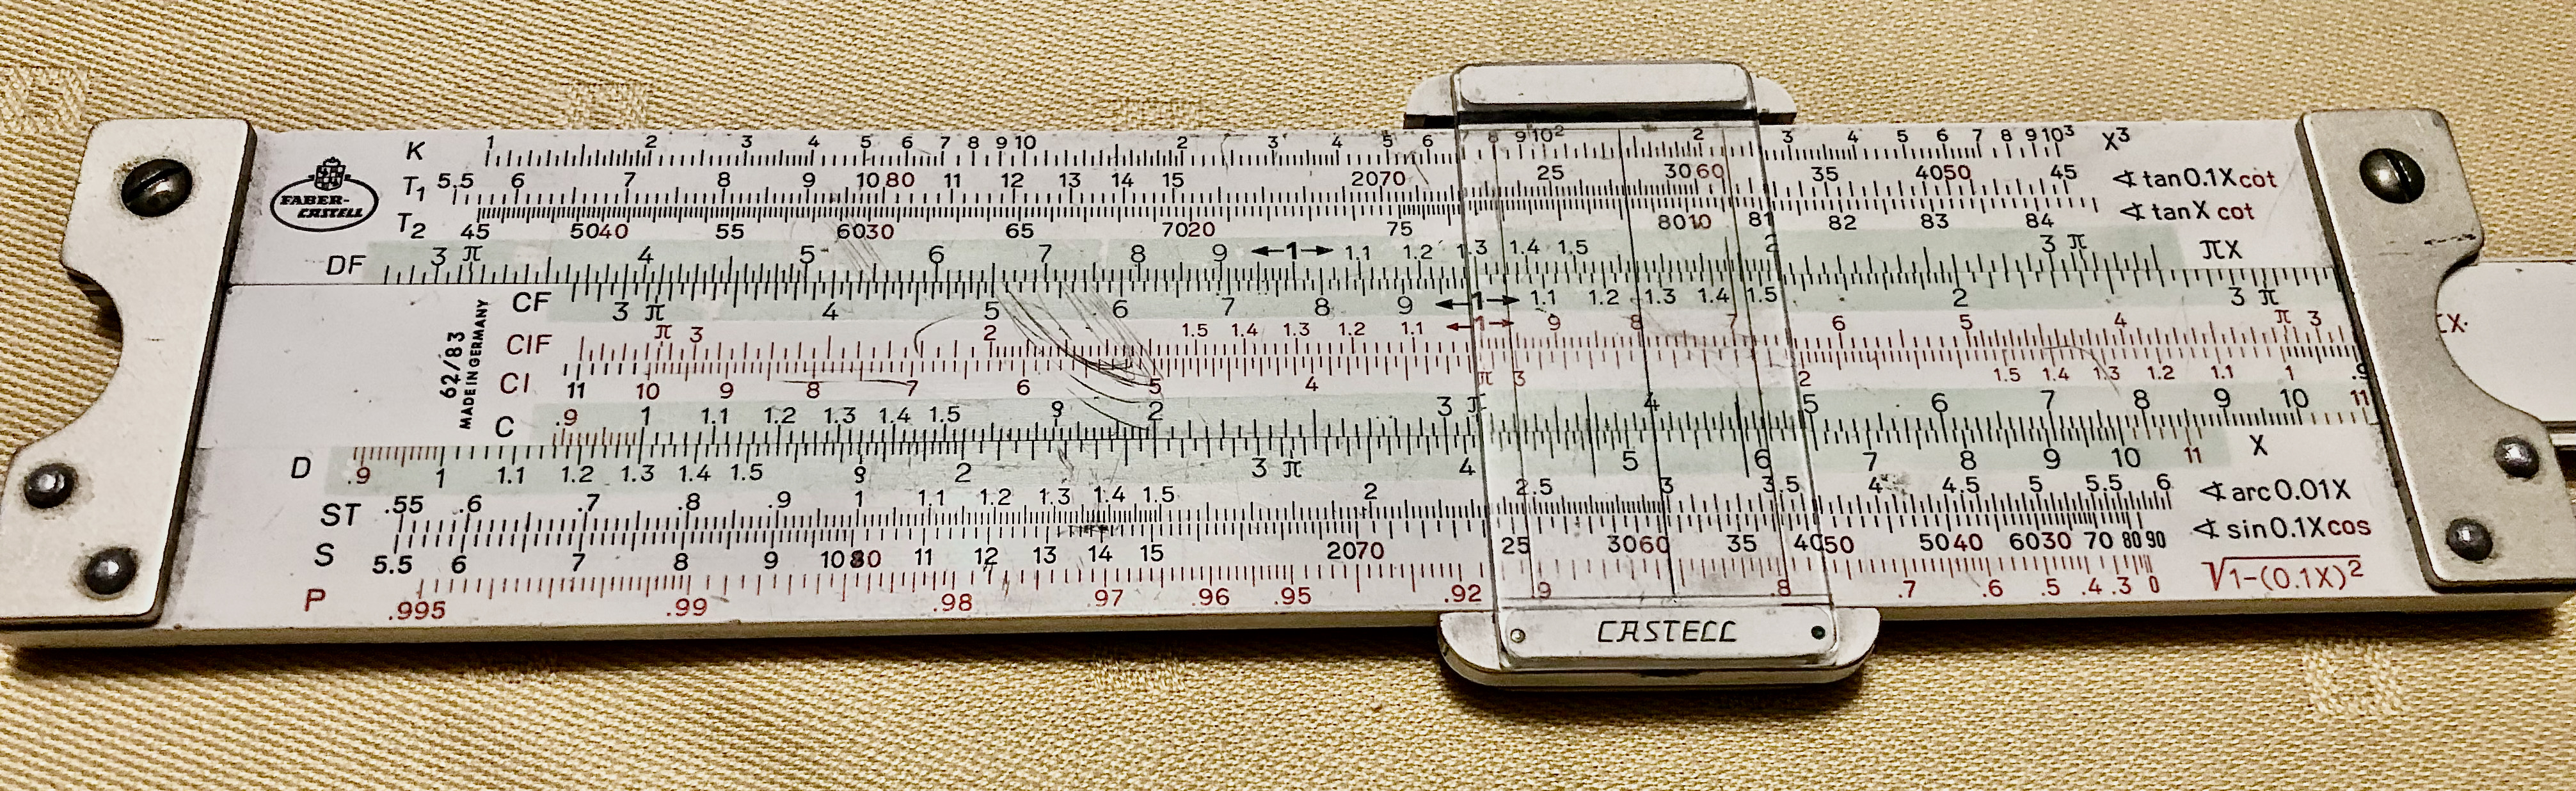
\includegraphics[scale=0.1]{IMG_1091.jpeg}
\end{center}

Räknestickan har en fast D-skala och en \emph{slid} med bland annat en likadan C-skala. Stickan ovan är inställd på multiplikationen ''$1.3 \cdot 4$''. C-skalans ''1''  ställs över ''1.3'' på D-skalan varefter löparstrecket skjuts till ''4'' på C-skalan och resultatet ''5.2'' avläses på D-skalan. Exakt samma inställning görs för divisionen $52/4$ där resultatet med siffrorna ''13'' avläses under C-skalans ''1''. Man kan också läsa av $5.2^3=140$ på den översta X$^3$-skalan. Exakta svaret är $140.608$ men närmevärdet $140$ duger i de flesta sammanhang. 

Slidens CI-skala är C-skalans inverterade värde och  DF-skalan D-skalans värde gånger $\pi$. På räknestickans baksida finns ytterligare skalor. Till exempel kan $\sqrt{x}$ beräknas genom att ställa in $x$ på D-skalan och läsa av resultatet på stickans baksida.

Man noterar att räknestickan bara ger siffrorna, och skiljer inte på $0.13$, $1.3$ eller $13~000$. Storleksordningarna får man göra bredvid eller i huvudet.

Det fanns också speciella räknestickor för olika yrkesområden. Man kan tänka sig en räknesticka för elektronik och beräkningar av kortslutningsström, resonansfrekvens hos kretsar med kondensatorer och spolar, serie- och parallellkopplingar av impedanser osv. Eller för vattenflöde genom rörledningar av viss längd och diameter givet visst tryck; beräkningar man är glad att slippa göra från grunden varje gång.

Mycket tid har ägnats åt att minimera risken för felavläsning av räknestickans skalor. Den kunskapen kan i dag nyttjas för att konstruera enkla och lättavlästa skalor.

\section{Lineära standardskala}

En \emph{standardskala} med värden mellan 0 och 10 cm med lätt avläsning är denna där skalstreck avsätts mot en \emph{stomlinje}:

\begin{center}
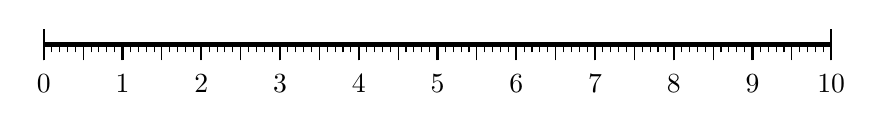
\begin{tikzpicture}[scale=1.0] %[xscale=1.3,yscale=1.3]
\draw[ultra thick] (0,0) --(10,0);
\foreach \x in {0,10} {
\draw[thick] (\x,-0.2) -- ( \x ,0.2);
}
\foreach \x in {0,1,...,10} {
\node at (\x, -0.5) {\pgfmathprintnumber[fixed,precision=1]{\x}}; 
\draw[thick] (\x,-0.2) -- ( \x ,0);
}
\foreach \x in {0,0.5,...,10} {
\draw[thin] (\x,-0.2) -- ( \x ,0);
}
\foreach \x in {0.0,0.1,...,10} {
\draw[thin] (\x,-0.1) -- ( \x ,0);
}
\end{tikzpicture}
\end{center}

Varje linjal har en skala som denna. Mer specifikt:

\begin{itemize}
\item Den har gradering under varje enhet (centimeter), 
\item däremellan 10 tunnare uppdelningar (millimeter) och, 
\item för att lättare hitta mittpunkten (5 mm) även ett längre tunt streck i denna punkt. 
\end{itemize}

Notera att skalans ändar markeras med genomgående vertikala streck för de yttersta graderingarna $0$ och $10$ \emph{enbart} om dessa finns med. 

För många fall räcker denna typ av gradering. Det går att betona på annat sätt utan att den känns förvirrande, till exempel

\begin{center}
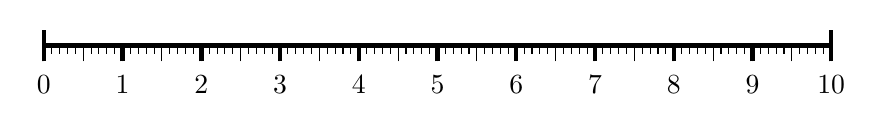
\begin{tikzpicture}[scale=1.0] %[xscale=1.3,yscale=1.3]
\draw[ultra thick] (0,0) --(10,0);
\foreach \x in {0,10} {
\draw[ultra thick] (\x,-0.2) -- ( \x ,0.2);
}
\foreach \x in {0,1,...,10} {
\node at (\x, -0.5) {\pgfmathprintnumber[fixed,precision=1]{\x}}; 
\draw[ultra thick] (\x,-0.2) -- ( \x ,0);
}
\foreach \x in {0,0.5,...,10} {
\draw[thin] (\x,-0.2) -- ( \x ,0);
}
\foreach \x in {0.0,0.1,...,10} {
\draw[thin] (\x,-0.1) -- ( \x ,0);
}
\end{tikzpicture}
\end{center}

eller till och med 

\begin{center}
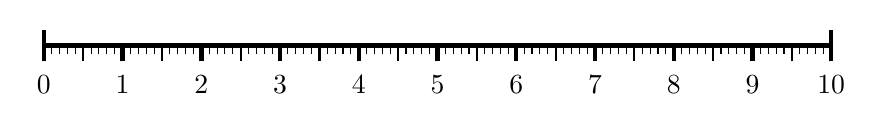
\begin{tikzpicture}[scale=1.0] %[xscale=1.3,yscale=1.3]
\draw[ultra thick] (0,0) --(10,0);
\foreach \x in {0,10} {
\draw[ultra thick] (\x,-0.2) -- ( \x ,0.2);
}
\foreach \x in {0,1,...,10} {
\node at (\x, -0.5) {\pgfmathprintnumber[fixed,precision=1]{\x}}; 
\draw[ultra thick] (\x,-0.2) -- ( \x ,0);
}
\foreach \x in {0,0.5,...,10} {
\draw[thick] (\x,-0.2) -- ( \x ,0);
}
\foreach \x in {0.0,0.1,...,10} {
\draw[thin] (\x,-0.1) -- ( \x ,0);
}
\end{tikzpicture}
\end{center}

Här utgörs de olika nivåerna av 1) skalstreck för numrerade enheter, 2) lika långa men tunnare skalstreck för mittpunkten (''5 mm'') mellan varje numrerad enhet och 3) något kortare, tunna skalstreck för varje millimeter.

Vid tillverkning av skalor och graderingar krävs ett visst mått av känsla för balans och syfte. Att blanda tjockare streck ''i fel ordning'' upplevs omedelbart störande, som denna:

\begin{center} 
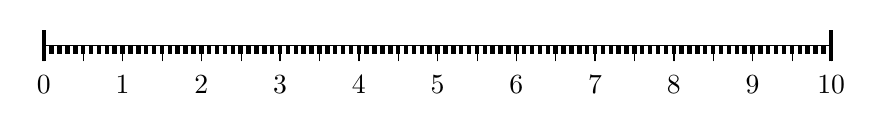
\begin{tikzpicture}[scale=1.0] %[xscale=1.3,yscale=1.3]
\draw[ultra thin] (0,0) --(10,0);
\foreach \x in {0,10} {
\draw[ultra thick] (\x,-0.2) -- ( \x ,0.2);
}
\foreach \x in {0,1,...,10} {
\node at (\x, -0.5) {\pgfmathprintnumber[fixed,precision=1]{\x}}; 
\draw[ thin] (\x,-0.2) -- ( \x ,0);
}
\foreach \x in {0,0.5,...,10} {
\draw[ultra thin] (\x,-0.2) -- ( \x ,0);
}
\foreach \x in {0.0,0.1,...,10.1} {
\draw[ultra thick] (\x,-0.1) -- ( \x ,0);
}
\end{tikzpicture}
\end{center}


Värre blir det med oproportionerliga siffror:

\begin{center} 
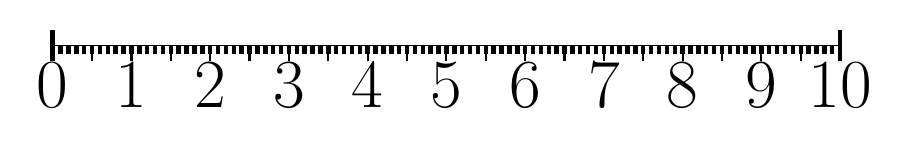
\begin{tikzpicture}[scale=1.0] %[xscale=1.3,yscale=1.3]
\draw[ultra thin] (0,0) --(10,0);
\foreach \x in {0,10} {
\draw[ultra thick] (\x,-0.2) -- ( \x ,0.2);
}
\foreach \x in {0,1,...,10} {
\node at (\x, -0.5) {\Huge\pgfmathprintnumber[fixed,precision=1]{\x}}; 
\draw[ thin] (\x,-0.2) -- ( \x ,0);
}
\foreach \x in {0,0.5,...,10} {
\draw[thick] (\x,-0.2) -- ( \x ,0);
}
\foreach \x in {0.0,0.1,...,10.1} {
\draw[ultra thick] (\x,-0.1) -- ( \x ,0);
}
\end{tikzpicture}
\end{center}


där skalans markeringar försvinner bakom de stora siffrorna.\footnote{En linjal som är tänkt att användas i dåligt ljus kan till exempel mycket väl ha stora siffror. Men detta är i så fall ett mycket speciellt användningsområde.}

\section{Avläsning}

Avläsningsprecisionen är ofta två till tre siffror även om skalstrecken antyder färre siffror. Se hur värdena nedan placerats även mellan de minsta skalstrecken. 

\begin{center}
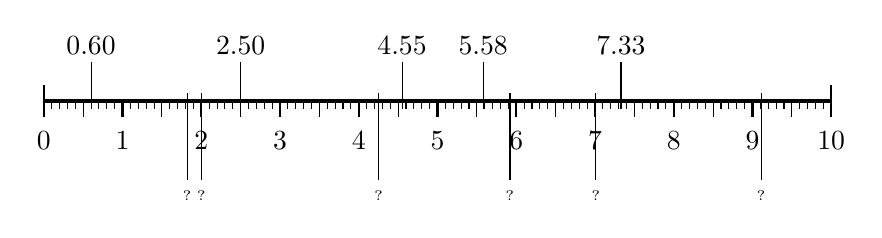
\begin{tikzpicture}[scale=1.0] %[xscale=1.3,yscale=1.3]
\draw[ultra thick] (0,0) --(10,0);
\foreach \x in {0,10} {
\draw[thick] (\x,-0.2) -- ( \x ,0.2);
}
\foreach \x in {0,1,...,10} {
\node at (\x, -0.5) {\pgfmathprintnumber[fixed,precision=1]{\x}}; 
\draw[thick] (\x,-0.2) -- ( \x ,0);
}
\foreach \x in {0,0.5,...,10} {
\draw[thin] (\x,-0.2) -- ( \x ,0);
}
\foreach \x in {0.0,0.1,...,10} {
\draw[thin] (\x,-0.1) -- ( \x ,0);
}

\foreach \x in {0.60, 2.50, 4.55, 5.58, 7.33} {
\node at (\x, 0.7) {{\x}}; 

\draw[thin] (\x,0.5) -- ( \x ,-0.1);
}

\foreach \x in {1.82, 2, 4.25, 5.92, 7.01, 9.11} {
\node at (\x, -1.2) {\tiny{?}}; 

\draw[thin] (\x,-1) -- ( \x ,0.1);
}

\end{tikzpicture}
\end{center}

Läs av de med ''?'' markerade strecken. Vilka värden med två decimaler motsvarar dessa? Eventuellt behövs förstoring av skalan men det är då enbart för att man ska kunna avläsa tydligt, det har inget med skalans egentliga upplösning att göra. 


\section{Förstoring hos skalor}

En skala kan behöva tillverkas för ett annat spann än en dekad (tiopotens). Det går utmärkt att ha en skala för värden mellan 2 och 5 till exempel:

\begin{center}
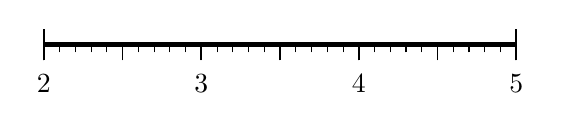
\begin{tikzpicture}[scale=1.0] %[xscale=1.3,yscale=1.3]
\draw[ultra thick] (4,0) --(10,0);
\foreach \x in {2,5} {
\draw[thick] (2*\x,-0.2) -- ( 2*\x ,0.2);
}
\foreach \x in {2,3,...,5} {
\node at (2*\x, -0.5) {\pgfmathprintnumber[fixed,precision=1]{\x}}; 
\draw[thick] (2*\x,-0.2) -- ( 2*\x ,0);
}
\foreach \x in {2,2.5,...,5} {
\draw[thin] (2*\x,-0.2) -- ( 2*\x ,0);
}
\foreach \x in {2.0,2.1,...,5} {
\draw[thin] (2*\x,-0.1) -- ( 2*\x ,0);
}
\end{tikzpicture}
\end{center}


Här ser man att intervallen mellan skalstrecken blivit större. Skalan är alltså både \emph{förstorad} jämfört med standardskalan och också avklippt mellan 2 och 5.

Generellt gäller att \emph{modulen}, dvs \emph{förstoringsgraden}, anges med $m$ och beräknas som \[m = \frac{L}{x_{max}-x_{min}} \]
där $L$ är skalans önskade längd och $x_{max}$ och $x_{min}$ skalans största och minsta värde. Ekvationen måste memoreras.

\startex {Ange modulen $m$ för en standardskala med längden 100 mm.}
För standardskalan är $L = 100$ mm, $x_{max}=10$ och $x_{min}=0$ dvs \[m = \frac{L}{x_{max}-x_{min}}= \frac{100}{10-0} = 10\, \textrm{mm/modul} \]


För skalan gäller alltså att skalstreck för värdet $n$ avsätts vid $m\cdot n$ mm från origo, dvs skalstrecken för \{0, 1, 2, 3, 4, 5, \ldots, 10\} avsätts vid \{0, 10, 20, 30, 40, 50, \ldots, 100\}~mm
\slutex


\startex {Ange modulen $m$ för en en skala med gränserna 2 och 5 och med  längden 60 mm.} Här är $L = 60$ mm, $x_{max}=5$ och $x_{min}=2$ dvs \[m = \frac{L}{x_{max}-x_{min}}= \frac{60}{5-2} = 20\, \textrm{mm/modul} \]

Skalan konstrueras med start i $2\cdot m = 2\cdot 20 = 40$ mm från origo och avslutas vid $5\cdot m = 5 \cdot 20=100$ mm. Skalans längd blir $100-40=60$ mm som önskat. 

\slutex

\section{Avläsning}

Med förstorad skala följer högre avläsningsprecision:

\begin{center}
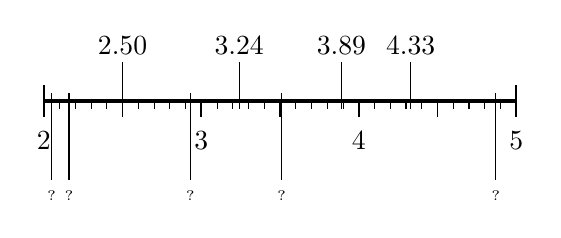
\begin{tikzpicture}[scale=1.0]
\draw[ultra thick] (4,0) --(10,0);
\foreach \x in {2,5} {
\draw[thick] (2*\x,-0.2) -- ( 2*\x ,0.2);
}
\foreach \x in {2,3,...,5} {
\node at (2*\x, -0.5) {\pgfmathprintnumber[fixed,precision=1]{\x}}; 
\draw[thick] (2*\x,-0.2) -- ( 2*\x ,0);
}
\foreach \x in {2,2.5,...,5} {
\draw[thin] (2*\x,-0.2) -- ( 2*\x ,0);
}
\foreach \x in {2.0,2.1,...,5} {
\draw[thin] (2*\x,-0.1) -- ( 2*\x ,0);
}


\foreach \x in {2.50, 3.24, 3.89, 4.33 } {
\node at (2*\x, 0.7) {{\x}}; 

\draw[thin] (2*\x,0.5) -- ( 2*\x ,-0.1);
}

\foreach \x in {2.05, 2.16, 2.93, 3.51, 4.87} {
\node at (2*\x, -1.2) {\tiny{?}}; 

\draw[thin] (2*\x,-1) -- ( 2*\x ,0.1);
}

\end{tikzpicture}
\end{center}

Det saknas ytterligare skalstreck för säker avläsning. Dessa \emph{kan} utföras genom att markera hälften av avstånden, 0.05, mellan de minsta skalstrecken 0.1:


\begin{center}
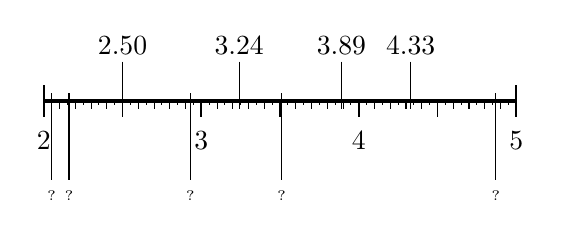
\begin{tikzpicture}[scale=1.0]
\draw[ultra thick] (4,0) --(10,0);
\foreach \x in {2,5} {
\draw[thick] (2*\x,-0.2) -- ( 2*\x ,0.2);
}
\foreach \x in {2,3,...,5} {
\node at (2*\x, -0.5) {\pgfmathprintnumber[fixed,precision=1]{\x}}; 
\draw[thick] (2*\x,-0.2) -- ( 2*\x ,0);
}
\foreach \x in {2,2.5,...,5} {
\draw[thin] (2*\x,-0.2) -- ( 2*\x ,0);
}
\foreach \x in {2.0,2.1,...,5} {
\draw[thin] (2*\x,-0.1) -- ( 2*\x ,0);
}

\foreach \x in {2.0,2.05,...,5} {
\draw[thin] (2*\x,-0.05) -- ( 2*\x ,0);
}

\foreach \x in {2.50, 3.24, 3.89, 4.33 } {
\node at (2*\x, 0.7) {{\x}}; 

\draw[thin] (2*\x,0.5) -- ( 2*\x ,-0.1);
}

\foreach \x in {2.05, 2.16, 2.93, 3.51, 4.87} {
\node at (2*\x, -1.2) {\tiny{?}}; 

\draw[thin] (2*\x,-1) -- ( 2*\x ,0.1);
}

\end{tikzpicture}
\end{center}

 eller \emph{endast undantagsvis} genom att dela upp i 0.02:
 
\begin{center}
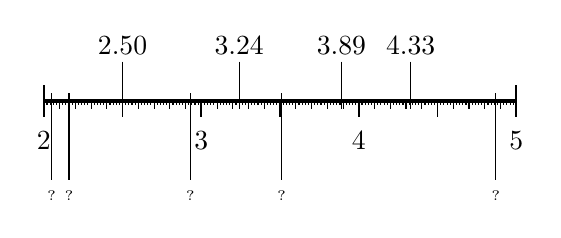
\begin{tikzpicture}[scale=1.0]
\draw[ultra thick] (4,0) --(10,0);
\foreach \x in {2,5} {
\draw[thick] (2*\x,-0.2) -- ( 2*\x ,0.2);
}
\foreach \x in {2,3,...,5} {
\node at (2*\x, -0.5) {\pgfmathprintnumber[fixed,precision=1]{\x}}; 
\draw[thick] (2*\x,-0.2) -- ( 2*\x ,0);
}
\foreach \x in {2,2.5,...,5} {
\draw[thin] (2*\x,-0.2) -- ( 2*\x ,0);
}
\foreach \x in {2.0,2.1,...,5} {
\draw[thin] (2*\x,-0.1) -- ( 2*\x ,0);
}

\foreach \x in {2.0,2.02,...,5} {
\draw[thin] (2*\x,-0.05) -- ( 2*\x ,0);
}

\foreach \x in {2.50, 3.24, 3.89, 4.33 } {
\node at (2*\x, 0.7) {{\x}}; 

\draw[thin] (2*\x,0.5) -- ( 2*\x ,-0.1);
}

\foreach \x in {2.05, 2.16, 2.93, 3.51, 4.87} {
\node at (2*\x, -1.2) {\tiny{?}}; 

\draw[thin] (2*\x,-1) -- ( 2*\x ,0.1);
}

\end{tikzpicture}
\end{center}

Denna icke-konventionella uppdelning med \emph{fyra} kan motiveras av att det annars skulle bli för tätt mellan skalstrecken, och får endast användas på den lägsta nivån.


\chapter{Dubbelskalor}
Dubbelskalor är skalor som avläses mot varann. De kan beskriva enkla funktionssamband eller mer komplicerade.

Genom lämplig skalning och med kunskap om ingående sifferområden kan praktiska dubbelskalor med tillräcklig precision för många tillämpningar tillverkas. Även en liten och därmed enbart ungefärlig dubbelskala kan ge snabb överblick om ett värde är rimligt eller ej.

\section{Lineära dubbelskalor av typen $y(x)=ax+b$}
Dessa dubbelskalor innehåller sammanhängande värden förenade med en variabel. Exempel är  enhetsomvandlingar: tum till centimeter, grader Celsius till grader Fahrenheit, kronor till euro och så vidare. Den färdiga dubbelskalan kan användas för omvandling åt båda hållen.


\startex{Tillverka en dubbelskala för omvandling mellan tum och centimeter. Dubbelskalans gränser skall vara 0 och 25 cm och längden 14 cm. En tum är 25.4 mm. Markeringar för $\frac{1}{10}$-dels tum tillåts på tumskalan.}

Här behövs två skalor som skall avsättas mot samma stomlinje. Skalorna olika moduler beräknas sålunda:

\begin{itemize}
\item För centimeterskalan: Här är $L = 140$ mm, $x_{max}=25$  och $x_{min}=0$ dvs \[m_{cm} = \frac{L}{x_{max}-x_{min}}= \frac{140}{25-0} = 5.6\, \textrm{mm/cm} \]

\item För tumskalan: Här är $L = 140$ mm, $x_{max}=250/25.4=9.84$ tum och $x_{min}=0/25.4=0$ tum dvs \[m_{tum} = \frac{L}{x_{max}-x_{min}}= \frac{140}{9.84-0} = 14.22\, \textrm{mm/tum} \]
\end{itemize}

Mot en 140 mm stomlinje avsätts de olika skalorna, en på varje sida:

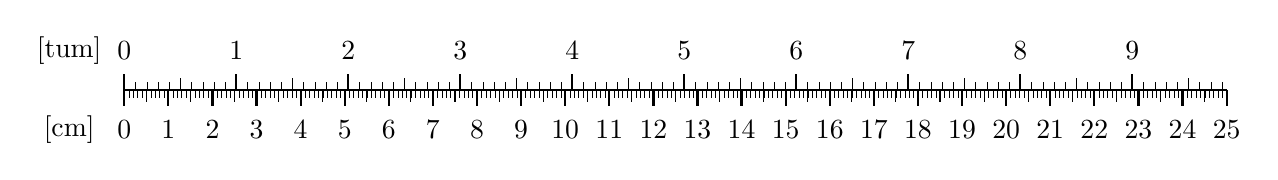
\begin{tikzpicture}[scale=1.0] %[xscale=1.3,yscale=1.3]

\node at (-0.7,-0.5) {[cm]};
\draw[ thick] (0,0) --(14,0);
\foreach \x in {0,1,...,25} {
\node at (0.56*\x, -0.5) {\pgfmathprintnumber[fixed,precision=1]{\x}}; 
\draw[thick] (0.56*\x,-0.2) -- ( 0.56*\x ,0);
}
\foreach \x in {0,0.5,...,25} {
\draw[ thin] (0.56*\x,-0.15) -- ( 0.56*\x,0);
}
\foreach \x in {0,0.1,...,25} {
\draw[ultra thin] (0.56*\x,-0.1) -- ( 0.56*\x ,0);
}

\node at (-0.7,0.5) {[tum]};
\foreach \x in {0,1,...,9.84} {
\node at (1.4224*\x, 0.5) {\pgfmathprintnumber[fixed,precision=1]{\x}}; 
\draw[thick] (1.4224*\x,0.2) -- ( 1.4224*\x ,0);
}
\foreach \x in {0,0.5,...,9.84} {
\draw[ thin] (1.4224*\x,0.15) -- ( 1.4224*\x,0);
}
\foreach \x in {0,0.1,...,9.84} {
\draw[ultra thin] (1.4224*\x,0.1) -- ( 1.4224*\x ,0);
}

\end{tikzpicture}

\slutex

Med dubbelskalan kan man nu snabbt konstatera att 3 tum på den övre skalan motsvarar 7.62 cm på den lägre. På liknande sätt kan 19 cm på den nedre avläsas som  7.48 tum på den övre. Med lite träning kan man läsa av skalorna med överraskande precision.




\startex{Tillverka en dubbelskala för att omvandla temperaturer mellan grader Celsius och grader Fahrenheit. Dubbelskalans gränser skall vara 36~$^\circ$C och 42~$^\circ$C och längden 10 cm. Sambandet kan skrivas \[\,^\circ F=\,^\circ C \cdot 1.8 + 32\].}

Här behövs två skalor som skall avsättas mot samma stomlinje. Skalornas olika $m$ beräknas sålunda:

\begin{itemize}

\item $m_{C}$: Här är $L = 100$ mm, $x_{max}=42\,^\circ C$  och $x_{min}=36\,^\circ C$ dvs 

\[m_C = \frac{L}{x_{max}-x_{min}}= \frac{100}{42-36} = 16.7\, \textrm{mm}/^\circ C \]

Här noteras att avståndet från origo till $x_{min}=36$ blir $36\cdot 16.7 = 600$ mm. För att placera ''36'' i origo måste alltså 600 subtraheras och de färdiga positionerna för siffra $ n \in \{36...42\}$ blir 

\[ n \cdot 16.7 -600\,\textrm{mm}.\]

\item $m_{F}$: Här är $L = 100$ mm, $x_{max}=42\cdot 1.8 + 32=107.6\,^\circ F$  och $x_{min}=36\cdot 1.8 + 32=96.8\,^\circ F$ dvs 

\[m_F = \frac{L}{x_{max}-x_{min}}= \frac{100}{107.6-96.8} = 9.26\, \textrm{mm}/^\circ F \]

På samma sätt som ovan måste $96.8\cdot 9.26 = 896.30$ subtraheras för att få punkten $96.8$ att sammanfalla med origo. För 
$n \in \{97...107\}$ blir avstånden 

\[ n \cdot 9.26 -896.30\,\textrm{mm}.\]

\end{itemize}

Mot en 100 mm stomlinje avsätts de olika skalorna, en på varje sida:


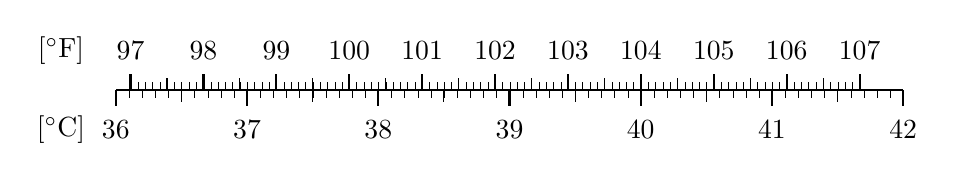
\begin{tikzpicture}[scale=1.0] %[xscale=1.3,yscale=1.3]

\draw[thick] (0,0) --(10,0);
\node at (-0.7,-0.5) {[$^\circ \textrm{C}$]};
\foreach \x in {36,...,42} {
\node at (1.6666*\x-60, -0.5) {\pgfmathprintnumber[fixed,precision=1]{\x}}; 
\draw[thick] (1.6666*\x-60,-0.2) -- ( 1.6666*\x-60 ,0);
}
\foreach \x in {36, 36.5,...,42} {
\draw[thin] (1.6666*\x-60,-0.15) -- ( 1.6666*\x-60,0);
}
\foreach \x in {36, 36.1,...,42} {
\draw[ultra thin] (1.6666*\x-60,-0.1) -- ( 1.6666*\x-60,0);
}

\node at (-0.7,0.5) {[$^\circ \textrm{F}$]};

\foreach \x in {97,98,...,107} {
\node at (0.925925*\x-89.63, 0.5) {\pgfmathprintnumber[fixed,precision=1]{\x}}; 
\draw[thick] (0.925925*\x-89.63,0.2) -- ( 0.925925*\x-89.63 ,0);
}
\foreach \x in {97,97.5,...,107} {
\draw[ thin] (0.925925*\x-89.63,0.15) -- ( 0.925925*\x-89.63,0);
}
\foreach \x in {97,97.1,...,107} {
\draw[ultra thin] (0.925925*\x-89.63,0.1) -- ( 0.925925*\x-89.63,0);
}

\end{tikzpicture}

En enkel kontrollpunkt är att $104\, ^\circ\textrm{F}$ motsvarar $40\, ^\circ\textrm{C}$ \emph{exakt}.

\chapter{Olineära skalor} 

En lineär skala kännetecknas av konstant modul, dvs ekvidistanta skalstreck. En lineär funktion av typen $y(x)=ax + b$ ger lineära skalor.

En olineär skala har inte konstant modul. Ett vanligt exempel är  logaritmfunktionen $y(x)=\lg x$ som är olineär. En logaritmisk standardskala för $x \in \{1,...,10\}$ och längden 140 mm konstrueras i princip på samma sätt som ovan men funktionen $y(x)=\lg x$ används.

\startex {Konstruera en logaritmisk standardskala för $x \in \{1,...,10\}$ och längden 140 mm.}

I detta fall är skalans funktion $y(x)=\lg x$ och $m$ beräknas med detta uttryck med $y(x_{max})$ och $y(x_{min})$. Tillvägagångssättet är för övrigt som förut:


\begin{itemize}
\item $m_{lg}$: Här är $L = 140$ mm, $y(x_{max})=\lg 10$  och $y(x_{min})=\lg 1$ dvs  \[m_{lg} = \frac{L}{y(x_{max})-y(x_{min})}= \frac{140}{1-0} = 140\, \textrm{mm/modul}\]
Då $y(1)=\lg 1=0$ sammanfaller skalans första skalstreck med origo och ingen förskjutning behövs. 
\end{itemize}


För att förtydliga konstruktionen anges här en linjal under den logaritmiska skalan:

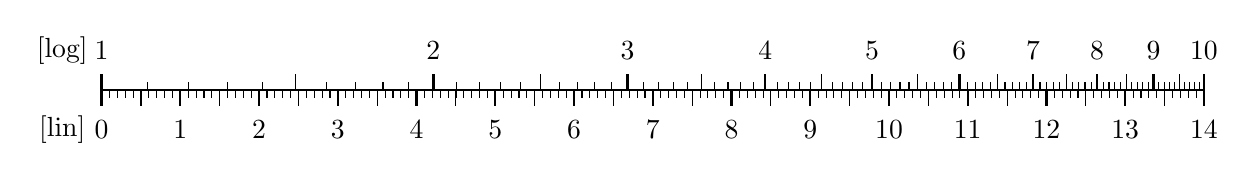
\begin{tikzpicture}[scale=1.0] %[xscale=1.3,yscale=1.3]
\draw[thick] (0,0) --(14,0);
\node at (-0.5,-0.5) {[lin]};

\foreach \x in {0,1,...,14} {
\node at (\x, -0.5) {\pgfmathprintnumber[fixed,precision=1]{\x}}; 
\draw[thick] (\x,-0.2) -- ( \x ,0);
}
\foreach \x in {0,0.5,...,14} {
\draw[thin] (\x,-0.2) -- ( \x ,0);
}
\foreach \x in {0.0,0.1,...,14} {
\draw[thin] (\x,-0.1) -- ( \x ,0);
}
% logskala
\node at (-0.5,0.5) {[log]};

\foreach \x in {1,2,...,10} {
\node at (14/ln 10 *ln \x, 0.5) {\pgfmathprintnumber[fixed,precision=1]{\x}}; 
\draw[thick] (14/ln 10 *ln \x,0.2) -- ( 14/ln 10 *ln \x ,0);
}
\foreach \x in {1,1.5,...,10} {
\draw[thin] (14/ln 10 *ln \x,0.2) -- ( 14/ln 10 *ln \x ,0);
}
\foreach \x in {1.0,1.1,...,10} {
\draw[thin] (14/ln 10 *ln \x,0.1) -- ( 14/ln 10 *ln \x ,0);
}
\end{tikzpicture}

Man ser att skalstrecken är väsentligt glesare från vänster och allt tätare åt höger. För att underlätta noggrann avläsning kan skalan kompletteras i den glesa delen:

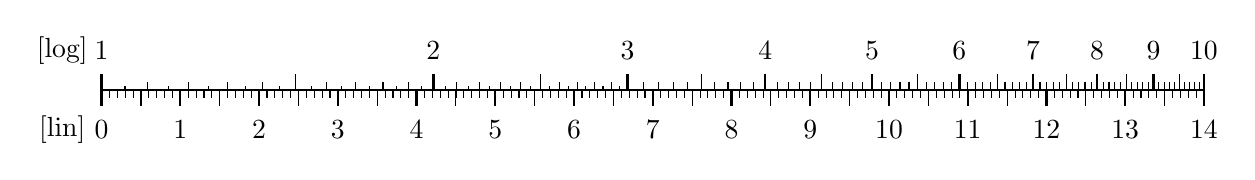
\begin{tikzpicture}[scale=1.0] %[xscale=1.3,yscale=1.3]
\draw[ thick] (-0,0) --(14,0);
\node at (-0.5,-0.5) {[lin]};

\foreach \x in {0,1,...,14} {
\node at (\x, -0.5) {\pgfmathprintnumber[fixed,precision=1]{\x}}; 
\draw[thick] (\x,-0.2) -- ( \x ,0);
}
\foreach \x in {0,0.5,...,14} {
\draw[thin] (\x,-0.2) -- ( \x ,0);
}
\foreach \x in {0.0,0.1,...,14} {
\draw[thin] (\x,-0.1) -- ( \x ,0);
}
% logskala
\node at (-0.5,0.5) {[log]};

\foreach \x in {1,2,...,10} {
\node at (14/ln 10 *ln \x, 0.5) {\pgfmathprintnumber[fixed,precision=1]{\x}}; 
\draw[thick] (14/ln 10 *ln \x,0.2) -- ( 14/ln 10 *ln \x ,0);
}
\foreach \x in {1,1.5,...,10} {
\draw[thin] (14/ln 10 *ln \x,0.2) -- ( 14/ln 10 *ln \x ,0);
}
\foreach \x in {1.0,1.1,...,10} {
\draw[thin] (14/ln 10 *ln \x,0.1) -- ( 14/ln 10 *ln \x ,0);
}
\foreach \x in {1.0,1.05,...,3} {
\draw[thin] (14/ln 10 *ln \x,0.05) -- ( 14/ln 10 *ln \x ,0);
}
\end{tikzpicture}

För att inte förväxla strecken för $1.1$ med $1.15$ osv måste de ytterligare tillagda markeringarna vara än mindre och någonstans når man skalans praktiska gräns för tillagda markeringar\footnote{De måste ju fortfarande synas liksom\ldots}. 

Fler än dessa skalstreck mellan 1 och 2 är svårmotiverade: 


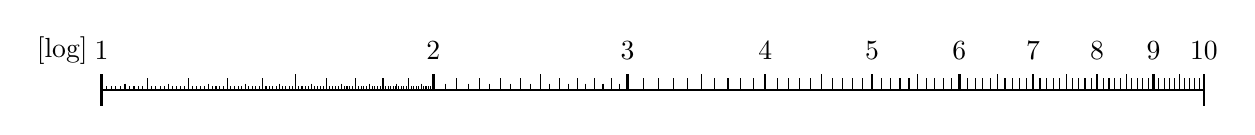
\begin{tikzpicture}[scale=1.0] %[xscale=1.3,yscale=1.3]
\draw[thick] (0,0) --(14,0);
\foreach \x in {0,14} {
\draw[thick] (\x,-0.2) -- ( \x ,0);
}

\node at (-0.5,0.5) {[log]};

\foreach \x in {1,2,...,10} {
\node at (14/ln 10 *ln \x, 0.5) {\pgfmathprintnumber[fixed,precision=1]{\x}}; 
\draw[thick] (14/ln 10 *ln \x,0.2) -- ( 14/ln 10 *ln \x ,0);
}
\foreach \x in {1,1.5,...,10} {
\draw[thin] (14/ln 10 *ln \x,0.2) -- ( 14/ln 10 *ln \x ,0);
}
\foreach \x in {1.0,1.1,...,10} {
\draw[thin] (14/ln 10 *ln \x,0.15) -- ( 14/ln 10 *ln \x ,0);
}
\foreach \x in {1.0,1.05,...,3} {
\draw[thin] (14/ln 10 *ln \x,0.08) -- ( 14/ln 10 *ln \x ,0);
}
\foreach \x in {1.0,1.01,...,2} {
\draw[thin] (14/ln 10 *ln \x,0.05) -- ( 14/ln 10 *ln \x ,0);
}
\end{tikzpicture}

Konstruktören får här göra en avvägning mellan praktisk användbarhet och önskad precision i avläsningen.


\section{Avläsning}

Avläsning görs på samma sätt som med lineära skalor men med större omsorg då skalan ändrar skalstreck och avstånd över hela skalan. Dessutom varierar avläsningsprecisionen längs skalan och blir sämre åt höger som ses nedan:


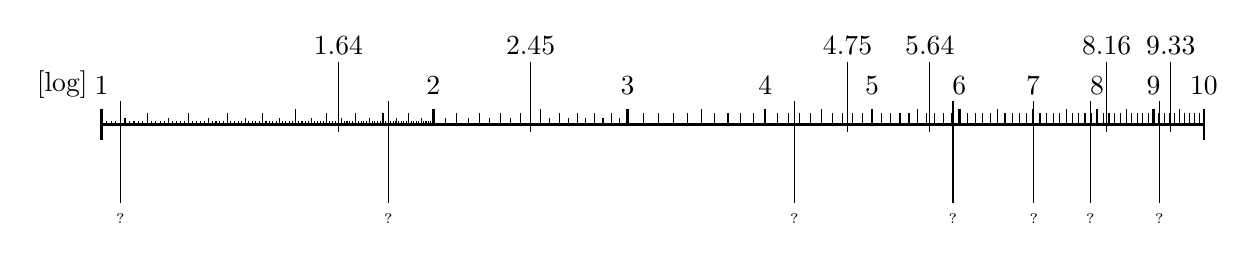
\begin{tikzpicture}[scale=1.0] %[xscale=1.3,yscale=1.3]
\draw[thick] (0,0) --(14,0);
\foreach \x in {0,14} {
\draw[thick] (\x,-0.2) -- ( \x ,0);
}

\node at (-0.5,0.5) {[log]};

\foreach \x in {1,2,...,10} {
\node at (14/ln 10 *ln \x, 0.5) {\pgfmathprintnumber[fixed,precision=1]{\x}}; 
\draw[thick] (14/ln 10 *ln \x,0.2) -- ( 14/ln 10 *ln \x ,0);
}
\foreach \x in {1,1.5,...,10} {
\draw[thin] (14/ln 10 *ln \x,0.2) -- ( 14/ln 10 *ln \x ,0);
}
\foreach \x in {1.0,1.1,...,10} {
\draw[thin] (14/ln 10 *ln \x,0.15) -- ( 14/ln 10 *ln \x ,0);
}
\foreach \x in {1.0,1.05,...,3} {
\draw[thin] (14/ln 10 *ln \x,0.08) -- ( 14/ln 10 *ln \x ,0);
}
\foreach \x in {1.0,1.01,...,2} {
\draw[thin] (14/ln 10 *ln \x,0.05) -- ( 14/ln 10 *ln \x ,0);
}


\foreach \x in {1.64, 2.45, 4.75, 5.64, 8.16,9.33} {
\node at (14/ln 10 *ln \x, 1) {{\x}}; 

\draw[thin] (14/ln 10 *ln \x,0.8) -- ( 14/ln 10 *ln \x ,-0.1);
}

\foreach \x in {1.04, 1.82, 4.25, 5.92, 7.01, 7.89, 9.11} {
\node at (14/ln 10 *ln \x, -1.2) {\tiny{?}}; 

\draw[thin] (14/ln 10 *ln \x,-1) -- ( 14/ln 10 *ln \x ,0.3);
}
\end{tikzpicture}


Avläsningsprecisionen kan ökas med ett noggrant val av skalans område. Ett mindre utsnitt av en logaritmisk skala ser närapå lineärt ut. Här är området mellan 7 och 10 valt (hela skalan mellan 1 och 10 är opraktiska 90 centimeter lång!):


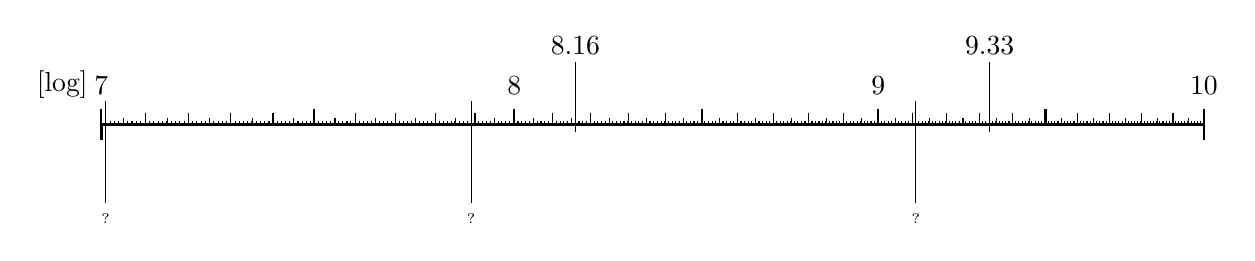
\begin{tikzpicture}[scale=1.0] %[xscale=1.3,yscale=1.3]
\draw[thick] (0,0) --(14,0);
\foreach \x in {0,14} {
\draw[thick] (\x,-0.2) -- ( \x ,0);
}

\node at (-0.5,0.5) {[log]};

\foreach \x in {7,...,10} {
\node at (90.3797/ln 10 *ln \x-76.3797, 0.5) {\pgfmathprintnumber[fixed,precision=1]{\x}}; 
\draw[thick] (90.3797/ln 10 *ln \x-76.3797,0.2) -- ( 90.3797/ln 10 *ln \x-76.3797 ,0);
}
\foreach \x in {7,7.5,...,10} {
\draw[thick] (90.3797/ln 10 *ln \x-76.3797,0.2) -- ( 90.3797/ln 10 *ln \x-76.3797 ,0);
}
\foreach \x in {7.0,7.1,...,10} {
\draw[thin] (90.3797/ln 10 *ln \x-76.3797,0.15) -- ( 90.3797/ln 10 *ln \x-76.3797,0);
}
\foreach \x in {7.0,7.05,...,10} {
\draw[thin] (90.3797/ln 10 *ln \x-76.3797,0.08) -- ( 90.3797/ln 10 *ln \x-76.3797,0);
}
\foreach \x in {7.0,7.01,...,10} {
\draw[thin] (90.3797/ln 10 *ln \x-76.3797,0.05) -- ( 90.3797/ln 10 *ln \x-76.3797,0);
}


\foreach \x in {8.16,9.33} {
\node at (90.3797/ln 10 *ln \x-76.3797, 1) {{\x}}; 

\draw[thin] (90.3797/ln 10 *ln \x-76.3797,0.8) -- ( 90.3797/ln 10 *ln \x-76.3797,-0.1);
}

\foreach \x in {7.01, 7.89,9.11} {
\node at (90.3797/ln 10 *ln \x-76.3797, -1.2) {\tiny{?}}; 

\draw[thin] (90.3797/ln 10 *ln \x-76.3797,-1) -- ( 90.3797/ln 10 *ln \x-76.3797,0.3);
}
\end{tikzpicture}

\section{Andra skalor}

Med metoderna ovan kan vilken skala som helst tillverkas så länge ett uttryck $y(x)$ finns tillgängligt.

\startex {Konstruera ett dubbelskala för funktionen $y(x)=3x^2+4$ med $x \in \{0,...,5\}$ med längden 100 mm.}

Först bestäms $m$ som förut:

\begin{itemize}
\item För standardskalan: Här är $L = 100$ mm, $x_{max}=5$  och $x_{min}=0$ dvs \\ \[m = \frac{L}{x_{max}-x_{min}}= \frac{100}{5-0} = 20\, \textrm{mm/modul}\]
\end{itemize}

Funktionsvärden för $y(x)$ avsättes på samma punkter och ger dessa skalor:

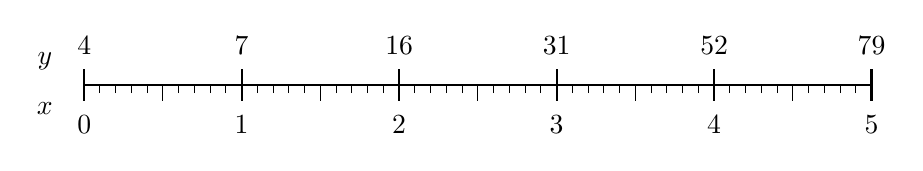
\begin{tikzpicture}[scale=1.0] %[xscale=1.3,yscale=1.3]
\draw[ thick] (0,0) --(10,0);
\node at (-0.5,-0.3) {$x$};

\foreach \x in {0,1,...,5} {
\node at (2*\x, -0.5) {\pgfmathprintnumber[fixed,precision=1]{\x}}; 
\draw[thick] (2*\x,-0.2) -- ( 2*\x ,0);
}
\foreach \x in {0,0.5,...,5} {
\draw[thin] (2*\x,-0.2) -- ( 2*\x ,0);
}
\foreach \x in {0.0,0.1,...,5} {
\draw[thin] (2*\x,-0.1) -- ( 2*\x ,0);
}

\node at (-0.5,0.3) {$y$};

\foreach \x in {0,1,...,5} {
\node at (2*\x , 0.5) {\pgfmathparse{3*\x*\x+4 }\pgfmathprintnumber\pgfmathresult}; 
\draw[thick] (2*\x  ,0.2) -- ( 2*\x  ,0);
}

\end{tikzpicture}


Man ser att den övre skalans värden, visserligen är korrekta $y$-värden för de givna $x$-värdena, men \emph{inte} sådana vi vill ha för enkel avläsning. Skalan skall vara lättavläst och alltså ange åtminstone 4, 10, 20, 30, 40, 50, 60, 70 och 79. För att kunna placera godtyckliga värden på övre skalan måste $x$ lösas ut ur ekvationen $y(x)=3x^2+4$ dvs 

 \[x(y)=\sqrt{\frac{y-4}{3}} \] och låta denna utgöra graderingen för $y \in {4, \ldots, 79}$:

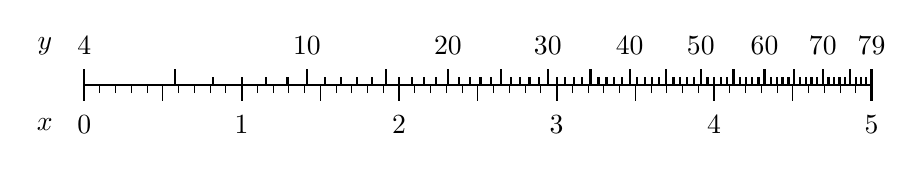
\begin{tikzpicture}[scale=1.0] %[xscale=1.3,yscale=1.3]
\draw[ thick] (0,0) --(10,0);
\node at (-0.5,-0.5) {$x$};

\foreach \x in {0,1,...,5} {
\node at (2*\x, -0.5) {\pgfmathprintnumber[fixed,precision=1]{\x}}; 
\draw[thick] (2*\x,-0.2) -- ( 2*\x ,0);
}
\foreach \x in {0,0.5,...,5} {
\draw[thin] (2*\x,-0.2) -- ( 2*\x ,0);
}
\foreach \x in {0.0,0.1,...,5} {
\draw[thin] (2*\x,-0.1) -- ( 2*\x ,0);
}


\node at (-0.5,0.5) {$y$};

\foreach \x in {10,20,...,79} {
\node at ( {2*sqrt((\x-4)/3)} , 0.5) {\pgfmathparse{\x}\pgfmathprintnumber\pgfmathresult}; 
\draw[thick] ({2*sqrt((\x-4)/3)} ,0.2) -- ( {2*sqrt((\x-4)/3)}  ,0);
}

\foreach \x in {4,79} {
\node at ( {2*sqrt((\x-4)/3)} , 0.5) {\pgfmathparse{\x}\pgfmathprintnumber\pgfmathresult}; 
\draw[thick] ({2*sqrt((\x-4)/3)} ,0.2) -- ( {2*sqrt((\x-4)/3)}  ,0);
}
\foreach \x in {5,10,...,79} {
\draw[thick] ({2*sqrt((\x-4)/3)} ,0.2) -- ( {2*sqrt((\x-4)/3)}  ,0);
}
\foreach \x in {6,7,...,79} {
\draw[thick] ({2*sqrt((\x-4)/3)} ,0.1) -- ( {2*sqrt((\x-4)/3)}  ,0);
}
\end{tikzpicture}

Vilket ger en mer praktisk skala som är lättare att avläsa och använda. 

\slutex

\chapter{Nomogram}

Genom att använda flera skalor konstrueras \emph{nomogram} genom vilka  \emph{addition} kan utföras. Nedan visas ett s k \emph{syftlinjesnomogram} för $f_3=f_1+f_2$. Genom att dra ett streck mellan skalorna $f_1$ och $f_2$ passerar strecket över $f_3$ på exakt den plats som anger summan. Denna princip är grunden för avläsning av alla nomogram. 

Med fördel används en \emph{genomskinlig} linjal för placering och avläsning då man får en uppfattning om punkternas omgivning och täthet på båda sidor om strecket. 

Avläsningsprecisionen bestäms av skalornas längd och gradering och kan utan större problem vara två eller tre värdesiffror. En skala av 30 cm:s längd tillåter cirka tre siffrors noggrannhet.

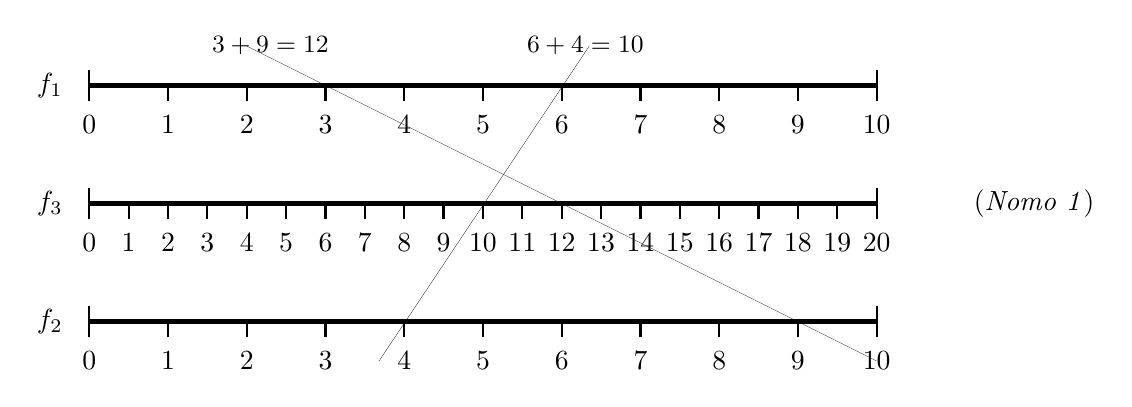
\begin{tikzpicture}[scale=1.0] 
\node at (-0.5,0) {$f_1$};
\node at (12,-1.5) {(\emph{Nomo 1})};

\draw[ultra thick] (0,0) --(10,0);
\foreach \x in {0,10} {
\draw[thick] (\x,-0.2) -- ( \x ,0.2);
}
\foreach \x in {0,1,...,10} {
\node at (\x, -0.5) {\pgfmathprintnumber[fixed,precision=1]{\x}}; 
\draw[thick] (\x,-0.2) -- ( \x ,0);
}
\node at (-0.5,-1.5) {$f_3$};

\draw[ultra thick] (0,-1.5) --(10,-1.5);
\foreach \x in {0,20} {
\draw[thick] (\x/2,-0.2-1.5) -- ( \x /2,0.2-1.5);
}
\foreach \x in {0,1,...,20} {
\node at (\x/2, -0.5-1.5) {\pgfmathprintnumber[fixed,precision=1]{\x}}; 
\draw[thick] (\x/2,-0.2-1.5) -- ( \x/2 ,0-1.5);
}

\node at (-0.5,-3) {$f_2$};
\draw[ultra thick] (0,-3) --(10,-3);
\foreach \x in {0,10} {
\draw[thick] (\x,-0.2-3) -- ( \x ,0.2-3);
}
\foreach \x in {0,1,...,10} {
\node at (\x, -0.5-3) {\pgfmathprintnumber[fixed,precision=1]{\x}}; 
\draw[thick] (\x,-0.2-3) -- ( \x ,0-3);
}

\node at (6.3, 0.5) {\small{$6+4=10$}};
\node at (2.3, 0.5) {\small{$3+9=12$}};

\draw[ultra thin] (3.68,-3.5) -- ( 6.35 ,0.5);
\draw[ultra thin] (10,-3.5) -- ( 2 ,0.5);

\end{tikzpicture}

Här visas tunna streck för additionerna $6+4$ och $3+9$. Genom att läsa av skalorna i annan ordning kan nomogrammet även användas för \emph{subtraktion}, här $10-6=4$ och $12-9=3$ osv.

Nomogrammets konstruktion  baserar sig på dimensionering av den övre och undre skalan som sedan leder till 

\begin{itemize}
\item mittenskalans skalvärden, \underline{och} 
\item placering mellan de övriga. 
\end{itemize}

\newpage
Avståndet mellan de tre skalorna benämns $a$ och $b$ och totala avståndet $c$ är då $a+b$:


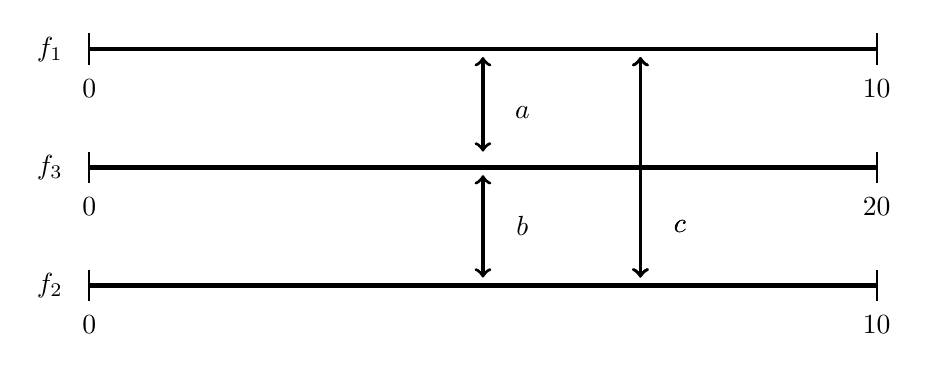
\begin{tikzpicture}[scale=1.0] %[xscale=1.3,yscale=1.3]
\node at (-0.5,0) {$f_1$};

\draw[ultra thick] (0,0) --(10,0);
\foreach \x in {0,10} {
\node at (\x, -0.5) {\pgfmathprintnumber[fixed,precision=1]{\x}}; 
\draw[thick] (\x,-0.2) -- ( \x ,0.2);
}

\draw [<->,very thick](5,-0.1) -- (5,-1.3);\node at (5.5, -0.8) {$a$};


\node at (-0.5,-1.5) {$f_3$};
\draw[ultra thick] (0,-1.5) --(10,-1.5);
\foreach \x in {0,20} {
\node at (\x/2, -0.5-1.5) {\pgfmathprintnumber[fixed,precision=1]{\x}}; 

\draw[thick] (\x/2,-0.2-1.5) -- ( \x /2,0.2-1.5);
}

\draw [<->,very thick](5,-1.6) -- (5,-2.9);\node at (5.5, -2.25) {$b$};

\node at (-0.5,-3) {$f_2$};
\draw[ultra thick] (0,-3) --(10,-3);
\foreach \x in {0,10} {
\node at (\x, -0.5-3) {\pgfmathprintnumber[fixed,precision=1]{\x}}; 
\draw[thick] (\x,-0.2-3) -- ( \x ,0.2-3);

\draw [<->,very thick](7,-0.1) -- (7,-2.9);\node at (7.5, -2.25) {$c$};

}
\end{tikzpicture}

Skalan $f_3$:s placering kan beräknas beroende på de yttre skalornas förstoring $m_a$ och $m_b$ enligt förhållandet

\[ \frac{a}{b}= \frac{m_a}{m_b}\]

Nomogrammet \emph{Nomo 1} ovan konstruerades med $m_1=m_2=10\, \textrm{mm/modul}$. $m_3$ bestäms precis som tidigare  

\begin{itemize}

\item med kännedom om  $f_3$:s största och minsta värde och \[ m_3=\frac{L}{x_{max}-x_{min}} \]
\item eller enligt formeln \[m_3=\frac{m_1m_2}{m_1+m_2}\].
\end{itemize}


Med $c=60$ mm beräknas både $a$ och $b$ till $15$ mm dvs $f_3$ placeras exakt mittemellan de övriga. 


\startex {Konstruera nomogrammet ovan med $m_1=20$ och $m_2=10$. $L=100\,\textrm{mm}$. $c=60\,\textrm{mm}$.}

Med $m_1=20\, \textrm{mm/modul}$ kommer första skalan, $f_1$, anta värden mellan 0 och 5, $m_2=10\, \textrm{mm/modul}$ ger att $f_2$ är oförändrad med tidigare.


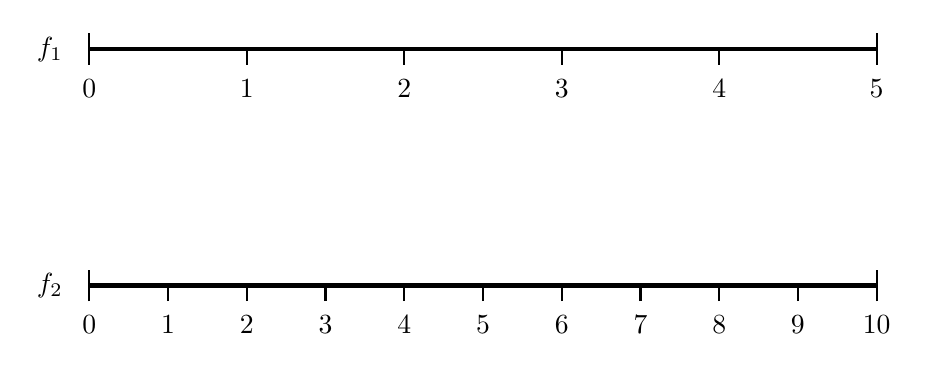
\begin{tikzpicture}[scale=1.0]
\node at (-0.5,0) {$f_1$};

\draw[ultra thick] (0,0) --(10,0);
\foreach \x in {0,5} {
\draw[thick] (2*\x,-0.2) -- ( 2*\x ,0.2);
}
\foreach \x in {0,1,...,5} {
\node at (2*\x, -0.5) {\pgfmathprintnumber[fixed,precision=1]{\x}}; 
\draw[thick] (2*\x,-0.2) -- ( 2*\x ,0);
}


\node at (-0.5,-3) {$f_2$};
\draw[ultra thick] (0,-3) --(10,-3);
\foreach \x in {0,10} {
\draw[thick] (\x,-0.2-3) -- ( \x ,0.2-3);
}
\foreach \x in {0,1,...,10} {
\node at (\x, -0.5-3) {\pgfmathprintnumber[fixed,precision=1]{\x}}; 
\draw[thick] (\x,-0.2-3) -- ( \x ,0-3);
}
\end{tikzpicture}

Skalan $f_3$ kan nu anta värden mellan 0 och 15 dvs $m_3=6.67$ mm/modul:

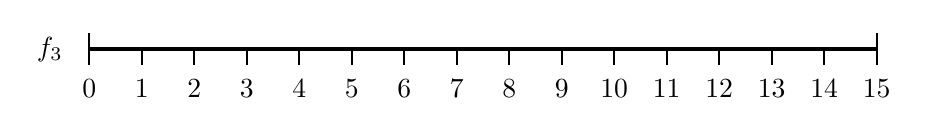
\begin{tikzpicture}[scale=1.0] %[xscale=1.3,yscale=1.3]
\node at (-0.5,0) {$f_3$};

\draw[ultra thick] (0,0) --(10,0);
\foreach \x in {0,15} {
\draw[thick] (2/3*\x,-0.2) -- ( 2/3*\x ,0.2);
}
\foreach \x in {0,1,...,15} {
\node at (2/3*\x, -0.5) {\pgfmathprintnumber[fixed,precision=1]{\x}}; 
\draw[thick] (2/3*\x,-0.2) -- ( 2/3*\x ,0);
}
\end{tikzpicture}

Enligt givna värden erhålls
\[ \frac{a}{b}= \frac{m_1}{m_2}=\frac{20}{10}= 2\]

dvs $a=2b$ och  $a+b=c$ ger $2b+b=c=60$ och  $b=20$, $a=40$. Skalan $f_3$ skall alltså placeras 40 mm från $f_1$, och det färdiga nomogrammet blir:\footnote{$\frac{a}{c}=\frac{40}{60}\approx 67\,\% $ från $f_1$-skalan.}

 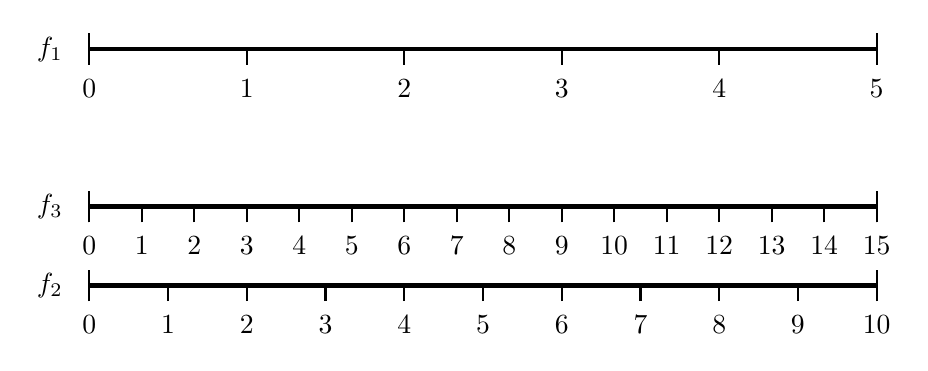
\begin{tikzpicture}[scale=1.0] %[xscale=1.3,yscale=1.3]
\node at (-0.5,0) {$f_1$};

\draw[ultra thick] (0,0) --(10,0);
\foreach \x in {0,5} {
\draw[thick] (2*\x,-0.2) -- ( 2*\x ,0.2);
}
\foreach \x in {0,1,...,5} {
\node at (2*\x, -0.5) {\pgfmathprintnumber[fixed,precision=1]{\x}}; 
\draw[thick] (2*\x,-0.2) -- ( 2*\x ,0);
}

\node at (-0.5,-2) {$f_3$};
\draw[ultra thick] (0,0-2) --(10,0-2);
\foreach \x in {0,15} {
\draw[thick] (2/3*\x,-0.2-2) -- ( 2/3*\x ,0.2-2);
}
\foreach \x in {0,1,...,15} {
\node at (2/3*\x, -0.5-2) {\pgfmathprintnumber[fixed,precision=1]{\x}}; 
\draw[thick] (2/3*\x,-0.2-2) -- ( 2/3*\x ,0-2);
}


\node at (-0.5,-3) {$f_2$};
\draw[ultra thick] (0,-3) --(10,-3);
\foreach \x in {0,10} {
\draw[thick] (\x,-0.2-3) -- ( \x ,0.2-3);
}
\foreach \x in {0,1,...,10} {
\node at (\x, -0.5-3) {\pgfmathprintnumber[fixed,precision=1]{\x}}; 
\draw[thick] (\x,-0.2-3) -- ( \x ,0-3);
}
\end{tikzpicture}

\slutex

På ovanstående sätt kan godtyckliga additions- och subtraktionsekvationer lösas.

\paragraph{Man kan notera} att det alltså finns ett samband mellan skalornas förstoring $m$ och placeringen av $f_3$-skalan. Med visst val av skalor kommer $f_3$-skalan \emph{för nära} någon av de övriga för att vara användbar. Innan man börjar konstruera ett nomogram måste man noggrant välja vilket talområde som verkligen behövs, och om det valda talområdet ger en acceptabel placering av $f_3$. Idealt ur avläsningssynpunkt är om $a=b$ dvs om $f_3$ placeras mittemellan ytterskalorna.

\section{Logaritmiska nomogram}

Logaritmiska nomogram utför samma addition eller subtraktion som tidigare men med logaritmiska skalor. Den operation som utförs är alltså som förut $f_3=f_1+f_2$ men då $f_i$ är logaritmiska får vi \[\lg f_3= \lg f_1 + \lg f_2\] dvs enligt logaritmlagarna egentligen multiplikationen \[f_3= f_1 \cdot f_2\]

I och med detta blir nomogrammet betydligt mer användbart.

\subsection{Nomogram för temperaturbestämning}
Från fysiken kan man få ett uttryck för den resistansändring en metall undergår vid uppvärmning. Tillämpat på en glödtråd i en lampa kan man med en mätt resistans vid rumstemperatur, $R_0$, och beräknad resistans, $R$, vid normal drift beräkna glödtrådens temperaturhöjning $\Delta T$ enligt formeln \[ \Delta T = \frac{R-R_0}{\alpha R_0} \,\, [^\circ\textrm{C}]\] där $\alpha$ är en materialkonstant. För volfram gäller $\alpha = 4.5\cdot 10^{-3}/^\circ$C.

Uttrycket är ännu inte på en form som lämpar sig för ett nomogram. Genom omskrivningen \[ \Delta T = \frac{R-R_0}{\alpha R_0} = \frac{1}{\alpha} \frac{R}{R_0}-\frac{1}{\alpha}\] och \[ \alpha \Delta T =  \frac{R}{R_0}-1\] till \[ 1+ \alpha \Delta T =  \frac{R}{R_0}\] fås efter logaritmering \[ \lg (1+ \alpha \Delta T) =  \lg R-\lg R_0\]

I denna form kan nomogrammet konstrueras. Termen ''$-\lg R_0$'' innebär att $R_0$-skalan skall ritas baklänges\footnote{Dvs från höger till vänster.}.

\startex{Konstruera ett nomogram enligt ovanstående formel av 150 mm längd med följande förutsättningar:
\begin{itemize}
\item $f_1: 15 \leq R \leq 25 \Omega$
\item $f_3: 1.5 \leq R_0 \leq 4 \Omega$
\item Glödtråden förutsätts vara av volfram
\end{itemize}

En direkt följd av de angivna gränserna är $611.11\,^\circ\textrm{C}\leq \Delta T \leq 3481.48\,^\circ\textrm{C}$.
}

Här behövs tre skalor för vardera $R, R_0$ och $\Delta T$. De konstrueras som tidigare: 

\begin{itemize}
\item[$f_1:$] \[m_1= \frac{150}{\lg 25- \lg 15}=676.14\,[\textrm{mm}/\lg \Omega]\]

Punkten 15 skall placeras i origo varför den sammanlagda funktionen blir \[f_1(R)=676.14\cdot \lg R -676.14\cdot \lg 15=676.14\cdot \lg R-795.20 \,[\textrm{mm}]\]

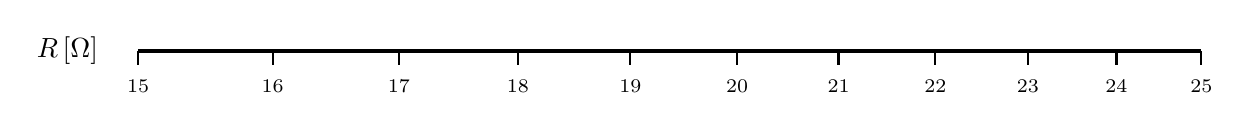
\begin{tikzpicture}[scale=0.9] %[xscale=1.3,yscale=1.3]
\draw[ultra thick] (0,0) --(15,0); \node at (-1,0) {$R\, [\Omega]$};
% R
\foreach \x in {15,...,25} {
\node at (67.614/ln 10 *ln \x -79.52, -0.5) {\scriptsize{\x}}; 
\draw[thick] (67.614/ln 10 *ln \x -79.52,-0.2) -- (67.614/ln 10 *ln \x -79.52,0);
}
\end{tikzpicture}



\item[$f_3:$] \[m_3= \frac{150}{\lg 4- \lg 1.5}=352.14\,[\textrm{mm}/\lg \Omega]\]  
\
Med resonemang som förut blir den sammanlagda funktionen  \[f_3(R_0)=352.14\cdot \lg R_0 -352.14\cdot \lg 1.5=352.14\cdot \lg R_0 - 62.01\,[\textrm{mm}]\].

Skalan ritas nu med origo till höger eller så subtraheras värdet från skallängden 150 mm: \[f_3 = 150-(352.14\cdot \lg R_0 - 62.01)= -352.14\cdot \lg R_0 + 212.01 \,[\textrm{mm}] \] .

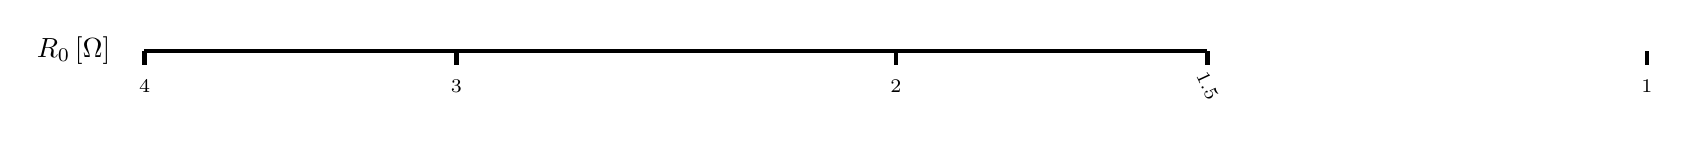
\begin{tikzpicture}[scale=0.9] %[xscale=1.3,yscale=1.3]
\draw[ultra thick] (0,-6.6) --(15,-6.6); \node at (-1,-6.6) {$R_0\, [\Omega]$};
%grovmodul med text
\foreach \x in {4,3,...,1} {
\node[rotate=0] at (-35.21/ln 10 *ln \x +21.2, -7.1) {\scriptsize{\x}}; 
\draw[ultra thick] (-35.21/ln 10 *ln \x +21.2,-6.8) -- (-35.21/ln 10 *ln \x +21.2,-6.6);
}
\foreach \x in {1.5} {
\node[rotate=-65] at (-35.21/ln 10 *ln \x +21.2, -7.1) {\scriptsize{\x}}; 
\draw[ultra thick] (-35.21/ln 10 *ln \x +21.2,-6.8) -- (-35.21/ln 10 *ln \x +21.2,-6.6);
}
\end{tikzpicture}


\item[{$f_2:$}] Skalan $m_2$ kan enligt tidigare beräknas på två sätt beroende på vilket som är lättast, antingen genom

\begin{itemize}
\item $m_2= \frac{m_1 \cdot m_3}{m_1 + m_3} = 231.55 \,[\textrm{mm}/\lg \Delta T]$ 

eller 

\item 
$m_2= \frac{150}{\lg (1+\alpha 3481.48) - \lg (1+ \alpha 611.11)}=231.55 \,[\textrm{mm}/\lg \Delta T]$.

Med resonemang som förut blir den sammanlagda funktionen inklusive förskjutning  \[f_2(\Delta T)=231.47\cdot \lg (1+\alpha \Delta T) - 231.47\cdot \lg (1+ \alpha 611.11)=231.47\cdot \lg \Delta T -132.87 \,[\textrm{mm}]\].
\end{itemize}


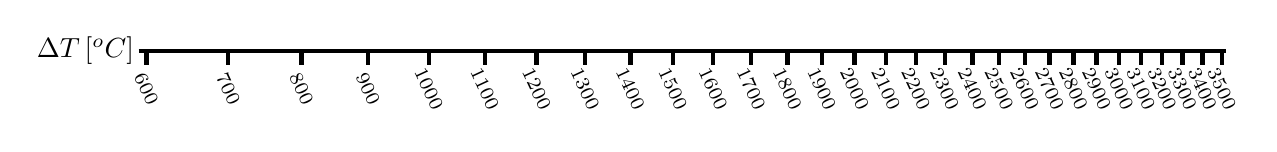
\begin{tikzpicture}[scale=0.9] %[xscale=1.3,yscale=1.3]
\draw[ultra thick] (-0.25,-4.34) --(15.1,-4.34); \node at (-1,-4.34) {$\Delta T \, [^o C]$};

\foreach \x in {600,700,...,3500} {
\node[rotate=-65] at ({23.14/ln 10 *ln (\x*0.0045+1) -13.29}, -4.88) {\scriptsize{\x}}; 
\draw[ultra thick] ({23.14/ln 10 *ln (\x*0.0045+1) -13.29},-4.54) -- ({23.14/ln 10 *ln (\x*0.0045+1) -13.29},-4.34);
}
\end{tikzpicture}

\end{itemize}

\paragraph{Skalavstånd} Återstår nu att bestämma avstånden $a$ och $b$. Ur de tidigare ekvationerna $\frac{a}{b}= \frac{m_1}{m_3}$ och $a+b =c$ fås, med $c=100\,\textrm{mm}$ 

\[ \frac{a}{b}= \frac{m_1}{m_3}\]

\[ b\frac{m_1}{m_3}+b = b(\frac{m_1}{m_3}+1)=c\] \[ b = \frac{c}{\frac{m_1}{m_3}+1} =  \frac{100}{\frac{676.14}{352.14}+1}=34.24\,\textrm{mm}\]

och

\[ a = c - b = 100 - 34.24= 65.75\,\textrm{mm} \]

Det resulterande nomogrammet med alla tre skalor försedda med finmarkeringar återges här i något förminskad form.

\fbox{
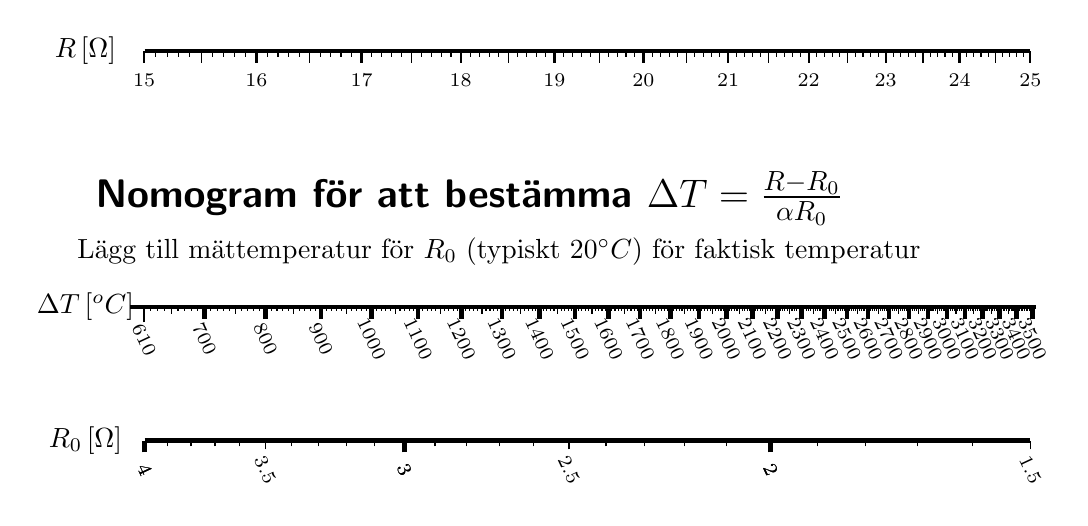
\begin{tikzpicture}[scale=0.75] %[xscale=1.3,yscale=1.3]

\draw[ultra thick] (0,0) --(15,0); \node at (-1,0) {$R\, [\Omega]$};
% R
\foreach \x in {15,...,25} {
\node at (67.614/ln 10 *ln \x -79.52, -0.5) {\scriptsize{\x}}; 
\draw[thick] (67.614/ln 10 *ln \x -79.52,-0.2) -- (67.614/ln 10 *ln \x -79.52,0);
}
\foreach \x in {15,15.1,...,25} {
\draw[thin] (67.614/ln 10 *ln \x -79.52,-0.1) -- (67.614/ln 10 *ln \x -79.52,0);
}
\foreach \x in {15,15.5,...,25} {
\draw[thin] (67.614/ln 10 *ln \x -79.52,-0.2) -- (67.614/ln 10 *ln \x -79.52,0);
}
\node at (5.5,-2.5){\Large\textsf{\textbf{Nomogram för att  bestämma $\Delta T=\frac{R-R_0}{\alpha R_0}$ }}};
%\node at (13,-2.5){$\alpha_{\texttt{volfram}}= 4.5 \cdot 10^{-3}/ ^\circ C$};
\node at (6,-3.4){Lägg till mättemperatur för $R_0$ (typiskt $20 ^\circ C$) för faktisk temperatur};

% temp

\draw[ultra thick] (-0.25,-4.34) --(15.1,-4.34); \node at (-1,-4.34) {$\Delta T \, [^o C]$};
\foreach \x in {700,800,...,3500} {
\node[rotate=-65] at ({23.14/ln 10 *ln (\x*0.0045+1) -13.29}, -4.88) {\scriptsize{\x}}; 
\draw[ultra thick] ({23.14/ln 10 *ln (\x*0.0045+1) -13.29},-4.54) -- ({23.14/ln 10 *ln (\x*0.0045+1) -13.29},-4.34);
}


%
\foreach \x in {610,620,...,3500} {
\draw[thin] ({23.14/ln 10 * ln (\x*0.0045+1) -13.29},-4.4) -- ({23.14/ln 10 *ln (\x*0.0045+1) -13.29},-4.34);
}

\foreach \x in {650,750,...,3400} {
\draw[thin] ({23.14/ln 10 * ln (\x*0.0045+1) -13.29},-4.45) -- ({23.14/ln 10 *ln (\x*0.0045+1) -13.29},-4.34);
}
\foreach \x in {1000,1500,...,3500} {
\draw[ultra thick] ({23.14/ln 10 * ln (\x*0.0045+1) -13.29},-4.54) -- ({23.14/ln 10 *ln (\x*0.0045+1) -13.29},-4.34);
}

\foreach \x in {610} {
\node[rotate=-65] at ({23.14/ln 10 *ln(611*0.0045+1) -13.29}, -4.9) {\scriptsize{\x}}; 
\draw[thick] ({23.14/ln 10 *ln(611*0.0045+1) -13.29},-4.6) -- ({23.14/ln 10 *ln(611*0.0045+1) -13.29},-4.34);
}

% R_0
% skala
\draw[ultra thick] (0,-6.6) --(15,-6.6); \node at (-1,-6.6) {$R_0\, [\Omega]$};
%grovmodul med text
\foreach \x in {4,3,...,1.5} {
\node[rotate=-65] at (-35.21/ln 10 *ln \x +21.2, -7.1) {\scriptsize{\x}}; 
\draw[ultra thick] (-35.21/ln 10 *ln \x +21.2,-6.8) -- (-35.21/ln 10 *ln \x +21.2,-6.6);

}
%Vissa tjocka streck
\foreach \x in {4,3.5,...,1.5} {
\node[rotate=-65] at (-35.21/ln 10 *ln \x +21.2, -7.1) {\scriptsize{\x}}; 

\draw[thin] (-35.21/ln 10 *ln \x +21.2,-6.75) -- (-35.21/ln 10 *ln \x +21.2,-6.6);
}
%Finmodul utan text
\foreach \x in {4,3.9,...,1.4} {

\draw[thin] (-35.21/ln 10 *ln \x +21.2,-6.7) -- (-35.21/ln 10 *ln \x +21.2,-6.6);
}

\end{tikzpicture}
}



\section{Känslighetsanalys med nomogram} En intressant sidoeffekt av ett nomogram är att man lätt kan få en uppfattning om hur känslig ett värde är för förändringar i de övriga. I nomogrammet för $\Delta T$ ovan ser man att temperaturen ändras snabbare till höger än till vänster.  

Man ser att en liten ändring i $R_0$ ger stor ändring i $\Delta T$, medan samma ändring i $R$ knappt ger någon ändring alls på  $\Delta T$-skalan. För ett korrekt värde på $\Delta T$ behövs alltså att $R_0$ är bestämd med hög noggrannhet. 

En följd av denna observation är att om $R_0=2.0\,\Omega$ är säker på till exempel $\pm 0.1 \Omega$ och $R=20 \,\Omega$ varierar $\Delta T$ med från $1900\,^\circ\textrm{C}$ till strax över $2100\,^\circ\textrm{C}$. Ett korrekt svar med högre precision än två siffror är inte rimligt. I talspråk  anges $2000\,^\circ\textrm{C}$, då det underförstås att det är ett närmevärde. 

%Mer korrekt anges  $2.0\cdot10^{3} \,^\circ\textrm{C}$.

\appendix
\chapter{Nomogram över $\Delta T$}
\pagenumbering{gobble}
\begin{center}
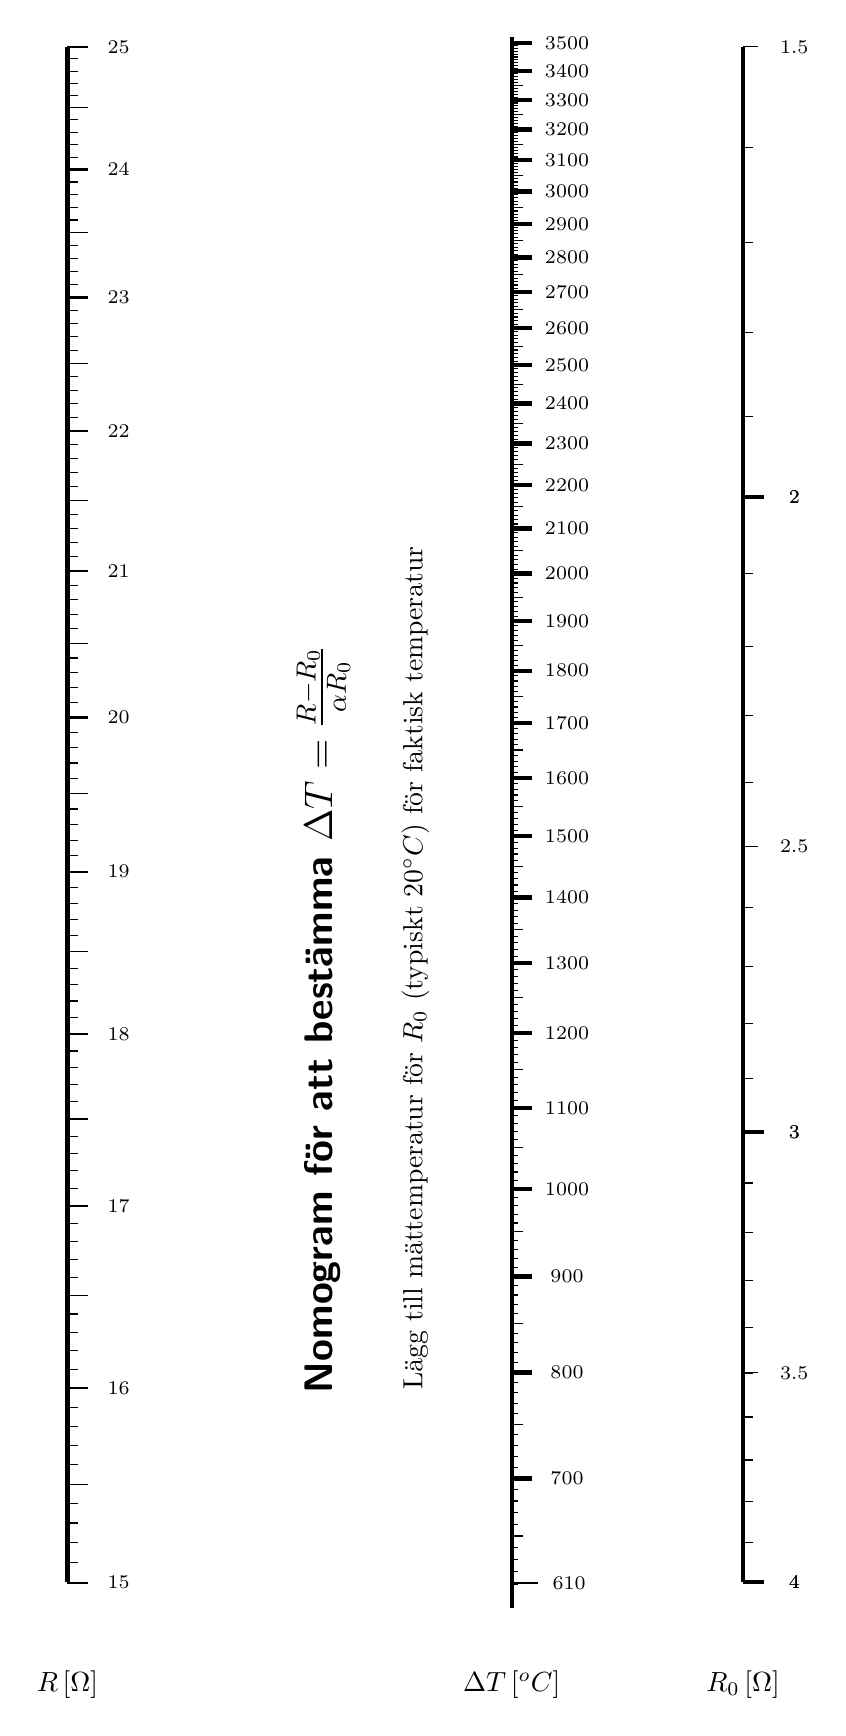
\begin{tikzpicture}[rotate=90, scale=1.3] %[xscale=1.3,yscale=1.3]

\draw[ultra thick] (0,0) --(15,0); \node at (-1,0) {$R\, [\Omega]$};
% R
\foreach \x in {15,...,25} {
\node at (67.614/ln 10 *ln \x -79.52, -0.5) {\scriptsize{\x}}; 
\draw[thick] (67.614/ln 10 *ln \x -79.52,-0.2) -- (67.614/ln 10 *ln \x -79.52,0);
}
\foreach \x in {15,15.1,...,25} {
\draw[thin] (67.614/ln 10 *ln \x -79.52,-0.1) -- (67.614/ln 10 *ln \x -79.52,0);
}
\foreach \x in {15,15.5,...,25} {
\draw[thin] (67.614/ln 10 *ln \x -79.52,-0.2) -- (67.614/ln 10 *ln \x -79.52,0);
}
\node at (5.5,-2.5)[rotate=90]{\Large\textsf{\textbf{Nomogram för att  bestämma $\Delta T=\frac{R-R_0}{\alpha R_0}$ }}};
%\node at (13,-2.5){$\alpha_{\texttt{volfram}}= 4.5 \cdot 10^{-3}/ ^\circ C$};
\node at (6,-3.4)[rotate=90]{Lägg till mättemperatur för $R_0$ (typiskt $20 ^\circ C$) för faktisk temperatur};

% temp

\draw[ultra thick] (-0.25,-4.34) --(15.1,-4.34); \node at (-1,-4.34) {$\Delta T \, [^o C]$};
\foreach \x in {700,800,...,3500} {
\node[rotate=0] at ({23.14/ln 10 *ln (\x*0.0045+1) -13.29}, -4.88) {\scriptsize{\x}}; 
\draw[ultra thick] ({23.14/ln 10 *ln (\x*0.0045+1) -13.29},-4.54) -- ({23.14/ln 10 *ln (\x*0.0045+1) -13.29},-4.34);
}


%
\foreach \x in {610,620,...,3500} {
\draw[thin] ({23.14/ln 10 * ln (\x*0.0045+1) -13.29},-4.4) -- ({23.14/ln 10 *ln (\x*0.0045+1) -13.29},-4.34);
}

\foreach \x in {650,750,...,3400} {
\draw[thin] ({23.14/ln 10 * ln (\x*0.0045+1) -13.29},-4.45) -- ({23.14/ln 10 *ln (\x*0.0045+1) -13.29},-4.34);
}
\foreach \x in {1000,1500,...,3500} {
\draw[ultra thick] ({23.14/ln 10 * ln (\x*0.0045+1) -13.29},-4.54) -- ({23.14/ln 10 *ln (\x*0.0045+1) -13.29},-4.34);
}

\foreach \x in {610} {
\node[rotate=0] at ({23.14/ln 10 *ln(611*0.0045+1) -13.29}, -4.9) {\scriptsize{\x}}; 
\draw[thick] ({23.14/ln 10 *ln(611*0.0045+1) -13.29},-4.6) -- ({23.14/ln 10 *ln(611*0.0045+1) -13.29},-4.34);
}

% R_0
% skala
\draw[ultra thick] (0,-6.6) --(15,-6.6); \node at (-1,-6.6) {$R_0\, [\Omega]$};
%grovmodul med text
\foreach \x in {4,3,...,1.5} {
\node[rotate=0] at (-35.21/ln 10 *ln \x +21.2, -7.1) {\scriptsize{\x}}; 
\draw[ultra thick] (-35.21/ln 10 *ln \x +21.2,-6.8) -- (-35.21/ln 10 *ln \x +21.2,-6.6);

}
%Vissa tjocka streck
\foreach \x in {4,3.5,...,1.5} {
\node[rotate=0] at (-35.21/ln 10 *ln \x +21.2, -7.1) {\scriptsize{\x}}; 

\draw[thin] (-35.21/ln 10 *ln \x +21.2,-6.75) -- (-35.21/ln 10 *ln \x +21.2,-6.6);
}
%Finmodul utan text
\foreach \x in {4,3.9,...,1.4} {

\draw[thin] (-35.21/ln 10 *ln \x +21.2,-6.7) -- (-35.21/ln 10 *ln \x +21.2,-6.6);
}

\end{tikzpicture}
\end{center}


\chapter{Théveninekvivalent}

Nomogrammet visar sambandet mellan tomgångsspänning $U_0$, inre resistans $R_i$ och kortslutningsström $I_k$ hos en Théveninekvivalent.

\begin{center}
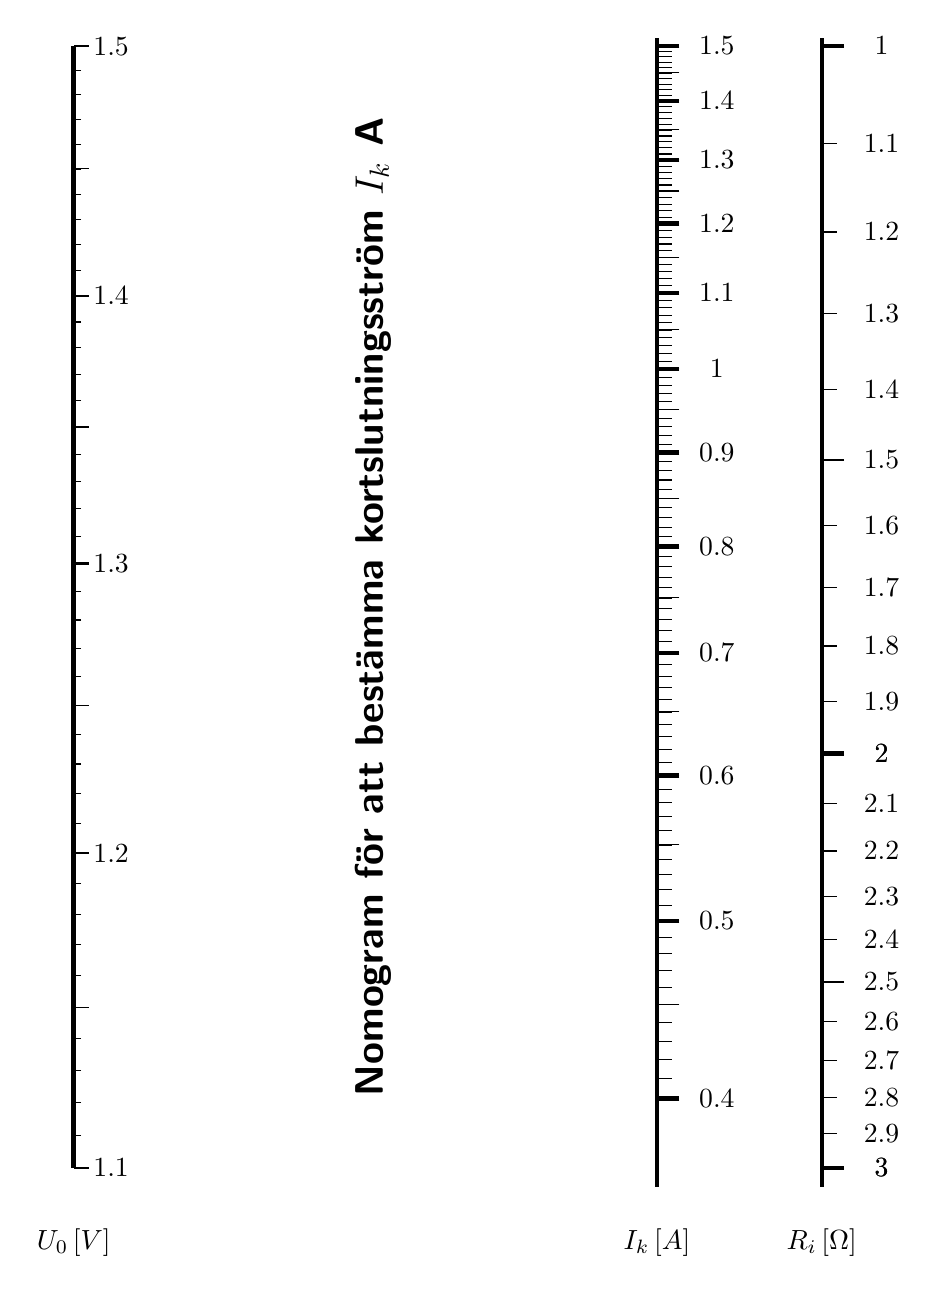
\begin{tikzpicture}[rotate=90, scale=0.95] %[xscale=1.3,yscale=1.3]
%
\draw[ultra thick] (0,0) --(15,0); \node at (-1,0) {$U_0\, [V]$};
% R
\foreach \x in {1.1,1.2,...,1.5} {
\node at (111.35976/ln 10 *ln \x -4.6094, -0.5) {\pgfmathprintnumber[fixed,precision=1]{\x}}; 
\draw[thick] (111.35976/ln 10 *ln \x -4.6094,-0.2) -- (111.35976/ln 10 *ln \x -4.6094,0);
}
\foreach \x in {1.11,1.12,...,1.5} {
\draw[thin] (111.35976/ln 10 *ln \x -4.6094,-0.1) -- (111.35976/ln 10 *ln \x -4.6094,0);
}
\foreach \x in {1.15,1.25,...,1.5} {
\draw[thin] (111.35976/ln 10 *ln \x -4.6094,-0.2) -- (111.35976/ln 10 *ln \x -4.6094,0);
}
\node at (7.5,-4)[rotate=90]{\Large\textsf{\textbf{Nomogram för att  bestämma kortslutningsström $I_k$ A} }};

% IK
\draw[ultra thick] (-0.25,-7.798) --(15.1,-7.798); 
\node at (-1,-7.798) {$I_k \, [A]$};

\foreach \x in {0.4,0.5,...,1.55} {
\node[rotate=0] at (24.51702/ln 10 *ln \x +10.683, -7.798-0.8) {\pgfmathprintnumber[fixed,precision=1]{\x}}; 
\draw[ultra thick] (24.51702/ln 10 *ln \x +10.683,-7.798-0.3) -- (24.51702/ln 10 *ln \x +10.683,-7.798);
}
\foreach \x in {0.41,0.42,...,1.5} {
\draw[thin] (24.51702/ln 10 *ln \x +10.683,-7.798-0.2) -- (24.51702/ln 10 *ln \x +10.683,-7.798);
}
\foreach \x in {0.45,0.50,...,1.5} {
\draw[thin] (24.51702/ln 10 *ln \x +10.683,-7.798-0.3) -- (24.51702/ln 10 *ln \x +10.683,-7.798);
}

% R_i
\draw[ultra thick] (-0.25,-10) --(15.1,-10); 
\node at (-1,-10) {$R_i \, [\Omega]$};

\foreach \x in {1,2,...,3} {
\node[rotate=0] at (-31.438/ln 10 *ln \x +15, -10-0.8) {\pgfmathprintnumber[fixed,precision=1]{\x}}; 
\draw[ultra thick] (-31.438/ln 10 *ln \x +15,-10-0.3) -- (-31.438/ln 10 *ln \x +15,-10);
}

\foreach \x in {1.1,1.2,...,3} {
\node[rotate=00] at (-31.438/ln 10 *ln \x +15, -10-0.8) {\pgfmathprintnumber[fixed,precision=1]{\x}};
\draw[thin] (-31.438/ln 10 *ln \x +15,-10-0.2) -- (-31.438/ln 10 *ln \x +15,-10);
}
\foreach \x in {1,1.5,...,3} {
\draw[thick] (-31.438/ln 10 *ln \x +15,-10-0.3) -- (-31.438/ln 10 *ln \x +15,-10);
}

\end{tikzpicture}
\end{center}




\chapter{Dubbelskalor}

\Large\textbf{\textsf{Termometer}} För att jämföra kroppstemperatur i grader Celsius och grader Fahrenheit är följande praktisk. Färgmarkeringen överensstämmer med normal temperatur, förhöjd temperatur och feber.

\vspace{7mm}

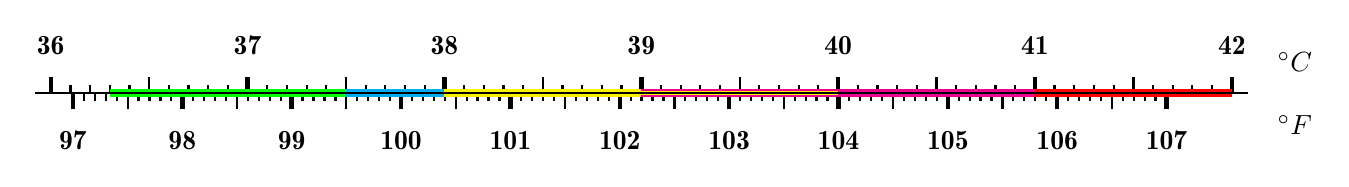
\begin{tikzpicture}[scale=1.0] %[xscale=1.4,yscale=1.3] för feber Celsius till Fahrenheit.\\

\draw[thick] (0,0) --(15.4,0); 
\node at (16,0.4) {$^\circ C$};
\node at (16,-0.4) {$^\circ F$};

\foreach \x in {36,37,...,42}{
	\node at (\x*15/6-89.8,0.6)  {\textbf{\x}}; 
	\draw[ultra thick] (\x*15/6-89.8,0.2) -- (\x*15/6-89.8,0);
}
\foreach \x in {36.1,36.2,...,42}	\draw[thick] (\x*15/6-89.8,0.1) -- (\x*15/6-89.8,0);
\foreach \x in {36.5,37.5,...,41.5}   \draw[thick] (\x*15/6-89.8,0.2) -- (\x*15/6-89.8,0);

\foreach \x in {97,98,...,107}{
	\node at (\x*15/10.8-134.24,-0.6) {\textbf{\x}};
	\draw[ultra thick] (\x*15/10.8-134.24,-0.2) -- (\x*15/10.8-134.24,0);
}

\foreach \x in {97.1,97.2,...,107}{
	\draw[thick] (\x*15/10.8-134.24,-0.1) -- (\x*15/10.8-134.24,0);
}

\foreach \x in {97.5,98.5,...,107}{
	\draw[thick] (\x*15/10.8-134.24,-0.2) -- (\x*15/10.8-134.24,0);
}

%subfebril

\draw[green,  very thick] (36.3*15/6-89.8,0.03) -- (37.5*15/6-89.8,0.03);
\draw[green,  very thick] (36.3*15/6-89.8,-0.03) -- (37.5*15/6-89.8,-0.03);

\draw[cyan,  very thick] (37.5*15/6-89.8,0.03) -- (38*15/6-89.8,0.03);
\draw[cyan,  very thick] (37.5*15/6-89.8,-0.03) -- (38*15/6-89.8,-0.03);

\draw[yellow,  very thick] (38*15/6-89.8,0.03) -- (40*15/6-89.8,0.03);
\draw[yellow,  very thick] (38*15/6-89.8,-0.03) -- (40*15/6-89.8,-0.03);

\draw[magenta,   thick] (39*15/6-89.8,0.04) -- (40*15/6-89.8,0.04);
\draw[magenta,   thick] (39*15/6-89.8,-0.04) -- (40*15/6-89.8,-0.04);


\draw[magenta, very thick] (40*15/6-89.8,0.03) -- (41*15/6-89.8,0.03);
\draw[magenta, very thick] (40*15/6-89.8,-0.03) -- (41*15/6-89.8,-0.03);


\draw[red,  very thick] (41*15/6-89.8,0.03) -- (42*15/6-89.8,0.03);
\draw[red,  very thick] (41*15/6-89.8,-0.03) -- (42*15/6-89.8,-0.03);


\end{tikzpicture}

\vspace{7mm}

\Large\textbf{\textsf{Matlagning}} Ugnstemperatur i amerikanska recept är angivna i grader Fahrenheit. Med denna dubbelskala översätts lätt till grader Celsius. Typiska standardtemperaturer i i vardera skalan är angivna.

\vspace{7mm}


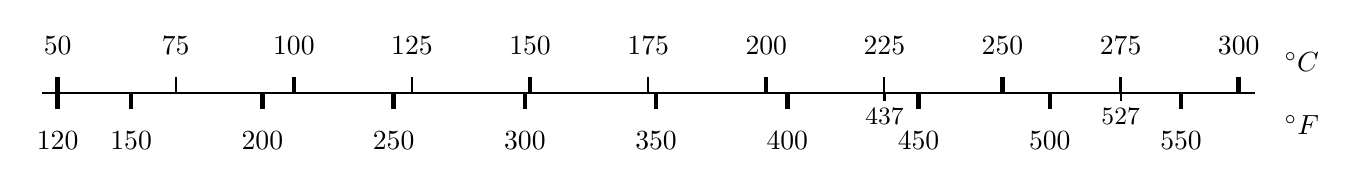
\begin{tikzpicture}[scale=1.0] %[xscale=1.4,yscale=1.3]


% densitet
\draw[thick] (0,0) --(15.4,0); 
\node at (16,0.4) {$^\circ C$};
\node at (16,-0.4) {$^\circ F$};


\foreach \x in {50,100,...,300}{
	\node at (\x*0.06-2.8,0.6)  {\x};  
	\draw[ultra thick] (\x*0.06-2.8,0.2) -- (\x*0.06-2.8,0);
}
\foreach \x in {75,125,...,275}{
	\node at (\x*0.06-2.8,0.6)  {\x};  
	\draw[thick] (\x*0.06-2.8,0.2) -- (\x*0.06-2.8,0);
}

\foreach \x in {150,200,...,550}{
	\node at (\x*6/180-3.8667,-0.6)  {\x}; 
	\draw[ultra thick] (\x*6/180-3.8667,-0.2) -- (\x*6/180-3.8667,0);
}
\node at (0.2,-0.6)  {120}; \draw[ultra thick] (0.2,-0.2) -- (0.2,0);
\node at (10.7,-0.3) {\small{437}}; \draw[thick] (10.7,-0.1) -- (10.7,0);
\node at (13.7,-0.3) {\small{527}}; \draw[thick] (13.7,-0.1) -- (13.7,0);


\end{tikzpicture}

\vspace{7mm}

\Large\textbf{\textsf{Mäsktemperatur}} Vid mäskning av malt vid öltillverkning används olika mäsktemperaturer. Optimala temperaturområden för   enzymerna $\alpha$- och $\beta$-amylas anges  med röd respektive grön markering.


\vspace{7mm}

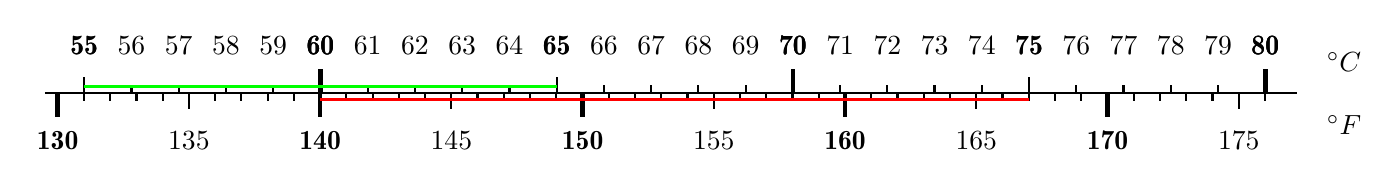
\begin{tikzpicture}[scale=1] %[xscale=1.4,yscale=1.3]
\draw[thick] (-0.5,0) --(15.4,0); 
\node at (16,0.4) {$^\circ C$};
\node at (16,-0.4) {$^\circ F$};

\foreach \x in {60,70,...,80}{
	\node at (\x*0.6-33,0.6)  {\text{\x}}; 
	\draw[ultra thick] (\x*0.6-33,0.3) -- (\x*0.6-33,0);
}


\foreach \x in {55,60,...,80}{
	\node at (\x*0.6-33,0.6)  {\textbf{\x}}; 
	\draw[thick] (\x*0.6-33,0.2) -- (\x*0.6-33,0);
}


\foreach \x in {55,56,...,80}{
	\node at (\x*0.6-33,0.6)  {\text{\x}}; 
	\draw[thick] (\x*0.6-33,0.1) -- (\x*0.6-33,0);
}

\foreach \x in {130,140,...,170}{
\node at (\x/3-43.67,-0.6)  {\textbf{\x}};
	\draw[ultra thick] (\x/3-43.67,-0.3) -- (\x/3-43.67,0);
}

\foreach \x in {135,145,...,175}{
\node at (\x/3-43.67,-0.6)  {\text{\x}};
	\draw[ thick] (\x/3-43.67,-0.2) -- (\x/3-43.67,0);
}

\foreach \x in {131,132,...,176}{
	\draw[thick] (\x/3-43.67,-0.1) -- (\x/3-43.67,0);
}


% beta amylase
\draw[green,  very thick] (55*0.6-33, 0.08) -- (65*0.6-33,0.08);
% alfa amylase
%\draw[cyan,  very thick] (60*0.6-33,0.03) -- (75*0.6-33,0.03);
\draw[red,  very thick] (60*0.6-33,-0.08) -- (75*0.6-33,-0.08);


\end{tikzpicture}

\chapter{Lin-log 1 dekad}

%%%%%%%%%%%%%%%%%%%%%%%%%%%%%%%%%%%%%%%%%%%%%%%%%%%%%%%%%%%
%linlog 1 decade START
%%%%%%%%%%%%%%%%%%%%%%%%%%%%%%%%%%%%%%%%%%%%%%%%%%%%%%%%%%
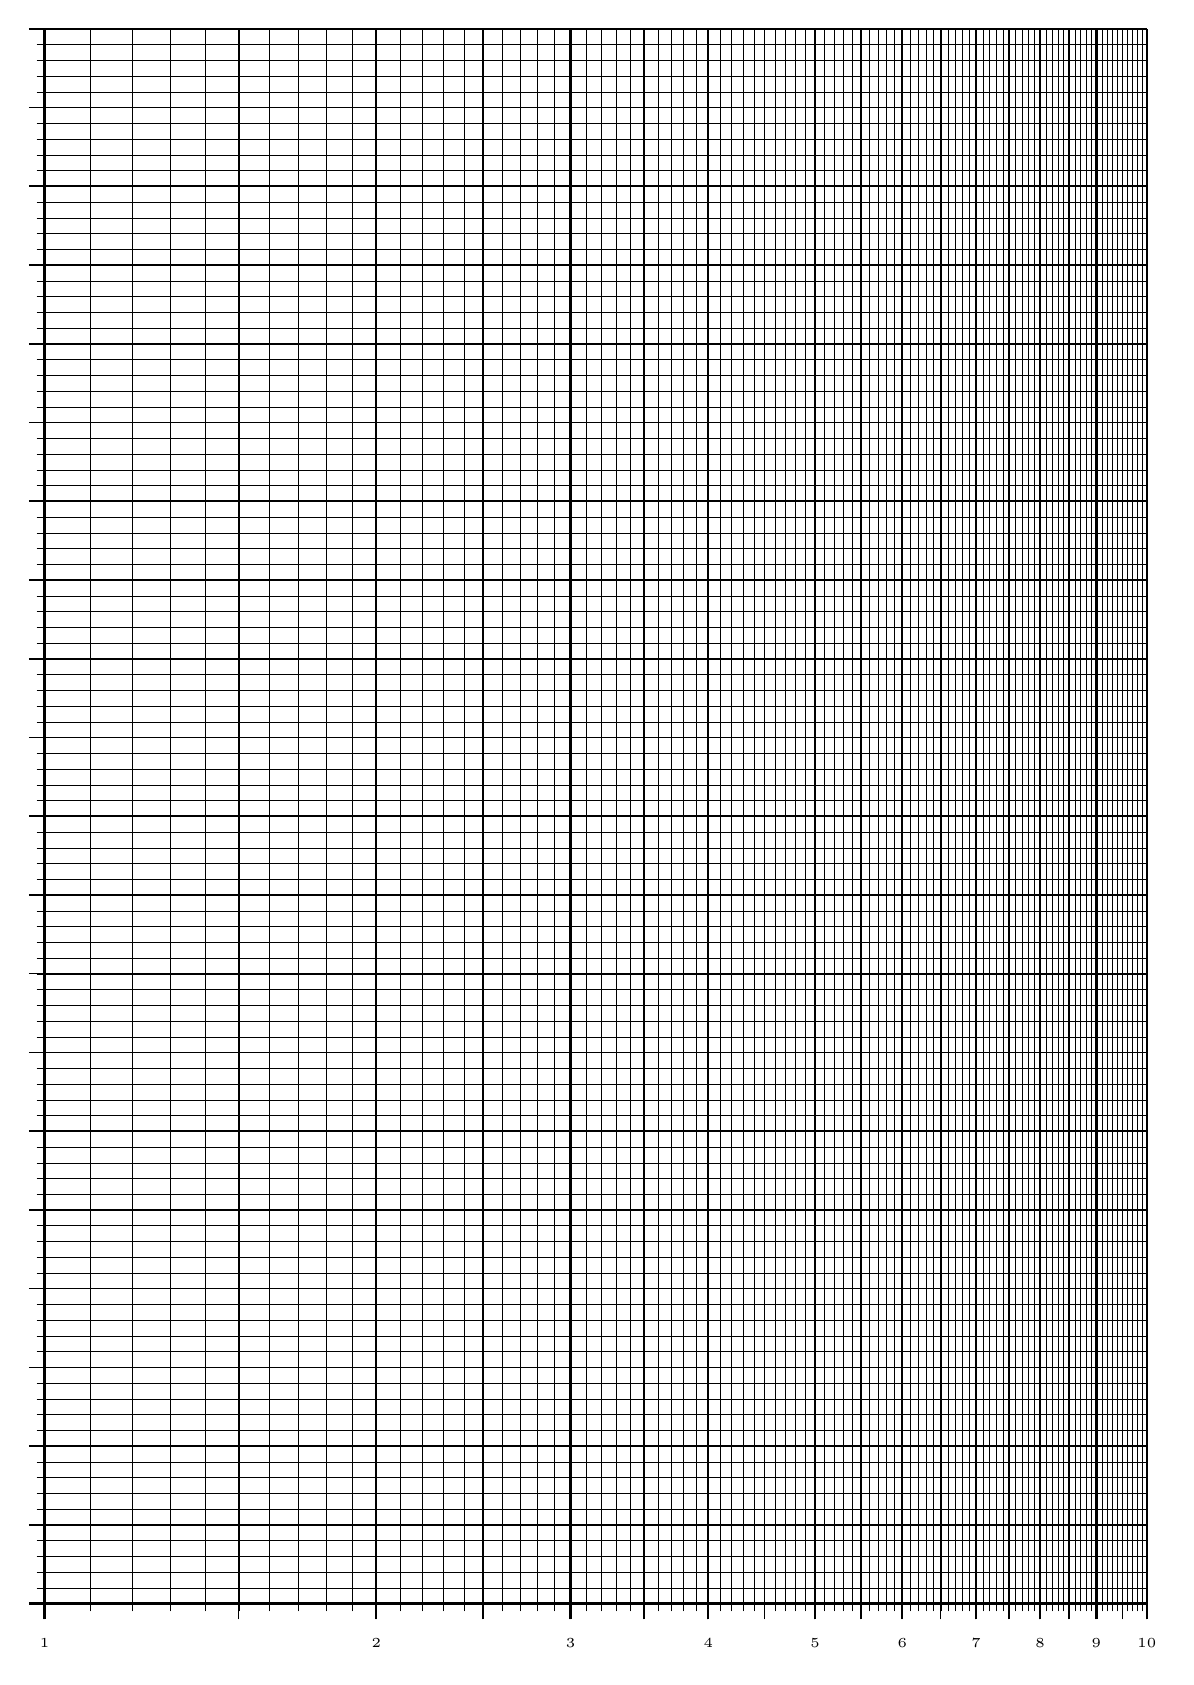
\begin{tikzpicture}[xscale=1,yscale=1] %[xscale=1.3,yscale=1.3]
\draw[thick] (-0.2,0) --(14,0);
\foreach \x in {1,2,...,10} {
\node at (14/ln 10 *ln \x, -0.5) {\tiny{\pgfmathprintnumber[fixed,precision=1]{\x}}}; 
\draw[thick] (14/ln 10 *ln \x,-0.2) -- ( 14/ln 10 *ln \x ,20);
}
\foreach \x in {1,1.5,...,10} {
\draw[semithick] (14/ln 10 *ln \x,-0.2) -- ( 14/ln 10 *ln \x ,20);
}
\foreach \x in {1.0,1.1,...,10} {
\draw[ultra thin] (14/ln 10 *ln \x,-0.1) -- ( 14/ln 10 *ln \x ,20);
}
\foreach \x in {0.2,0.4,...,20} {
\draw[ultra thin] (-0.1,\x) -- (14,\x);
}
\foreach \x in {1.0,2,...,20} {
\draw[semithick] (-0.2,\x) -- (14,\x);
}
\end{tikzpicture}
%%%%%%%%%%%%%%%%%%%%%%%%%%%%%%%%%%%%%%%%%%%%%%%%%%%%%%%%%%%
%linlog 1 decade END
%%%%%%%%%%%%%%%%%%%%%%%%%%%%%%%%%%%%%%%%%%%%%%%%%%%%%%%%%%



\chapter{Log-log 1 dekad}

%%%%%%%%%%%%%%%%%%%%%%%%%%%%%%%%%%%%%%%%%%%%%%%%%%%%%%%%%%%
%loglog 1 decade START
%%%%%%%%%%%%%%%%%%%%%%%%%%%%%%%%%%%%%%%%%%%%%%%%%%%%%%%%%%
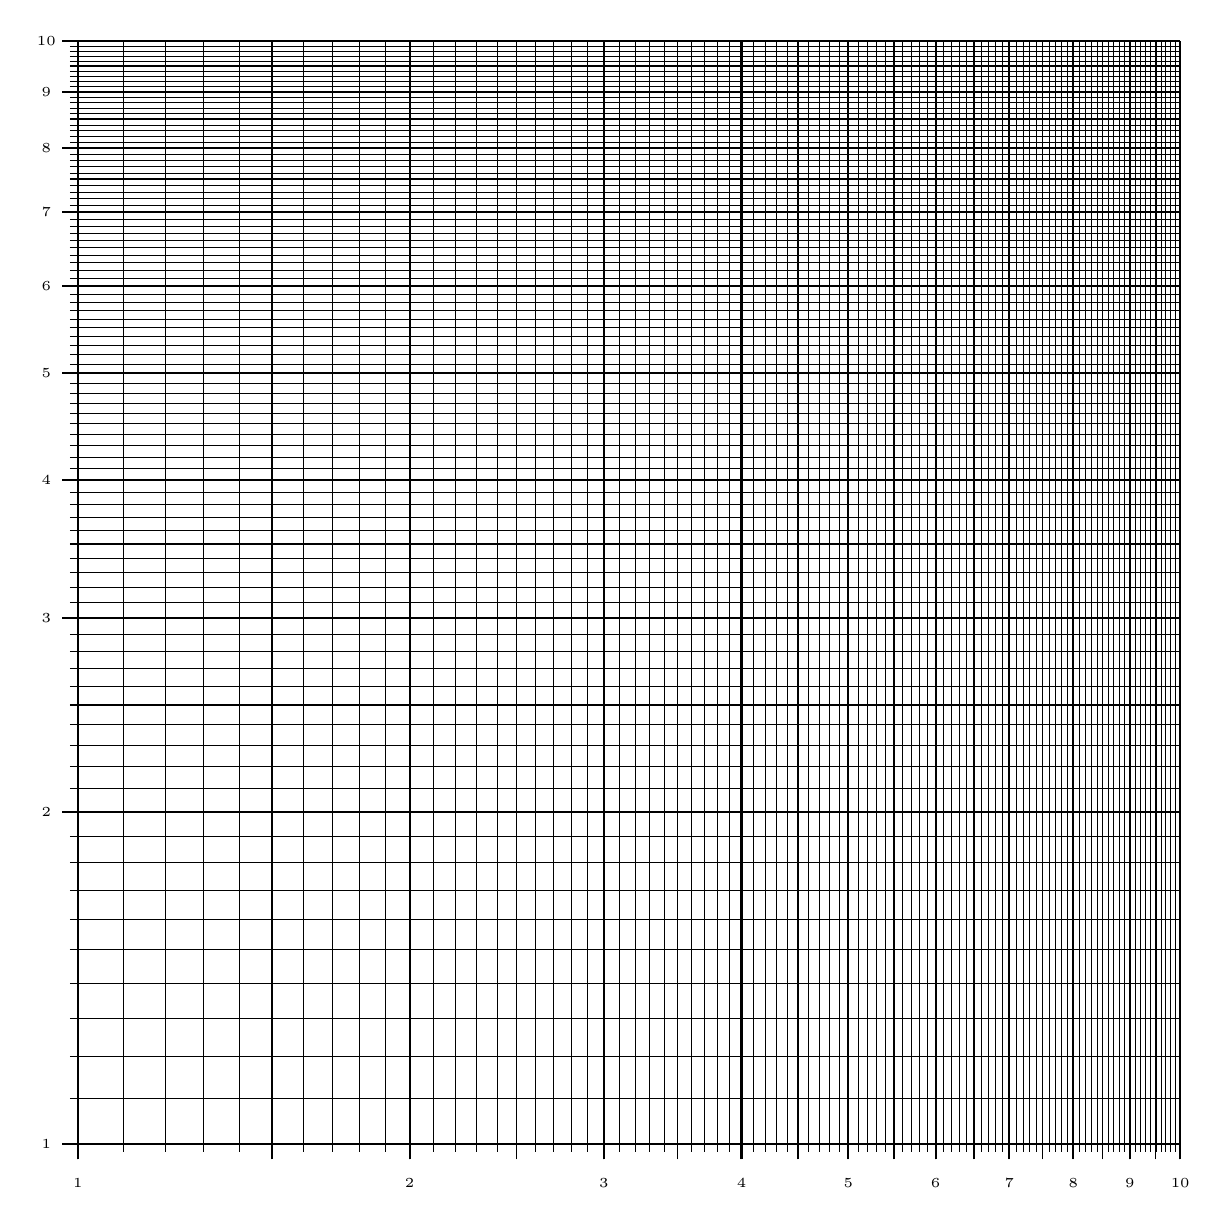
\begin{tikzpicture}[xscale=1,yscale=1] %[xscale=1.3,yscale=1.3]
\draw[ thick] (0,0) --(14,0);
\foreach \x in {1,2,...,10} {
\node at (14/ln 10 *ln \x, -0.5) {\tiny{\pgfmathprintnumber[fixed,precision=1]{\x}}}; 
\draw[thick] (14/ln 10 *ln \x,-0.2) -- ( 14/ln 10 *ln \x ,14);
}
\foreach \x in {1,1.5,...,10} {
\draw[semithick] (14/ln 10 *ln \x,-0.2) -- ( 14/ln 10 *ln \x ,14);
}
\foreach \x in {1.0,1.1,...,10} {
\draw[ultra thin] (14/ln 10 *ln \x,-0.1) -- ( 14/ln 10 *ln \x ,14);
}
\foreach \x in {1,2,...,10} {
\node at (-0.4, 14/ln 10 *ln \x) {\tiny{\pgfmathprintnumber[fixed,precision=1]{\x}}}; 
\draw[thick] (-0.2 ,14/ln 10 *ln \x) -- ( 14 ,14/ln 10 *ln \x);
}
\foreach \x in {1,1.5,...,10} {
\draw[semithick] (-0.1, 14/ln 10 *ln \x) -- ( 14, 14/ln 10 *ln \x);
}
\foreach \x in {1.0,1.1,...,10} {
\draw[ultra thin] (-0.1, 14/ln 10 *ln \x) -- ( 14, 14/ln 10 *ln \x);
}

\end{tikzpicture}
%%%%%%%%%%%%%%%%%%%%%%%%%%%%%%%%%%%%%%%%%%%%%%%%%%%%%%%%%%%
%loglog 1 decade END
%%%%%%%%%%%%%%%%%%%%%%%%%%%%%%%%%%%%%%%%%%%%%%%%%%%%%%%%%%


\chapter{Lin-log 3 dekader}



%%%%%%%%%%%%%%%%%%%%%%%%%%%%%%%%%%%%%%%%%%%%%%%%%%%%%%%%%%%
%linlog 3 decade START
%%%%%%%%%%%%%%%%%%%%%%%%%%%%%%%%%%%%%%%%%%%%%%%%%%%%%%%%%%
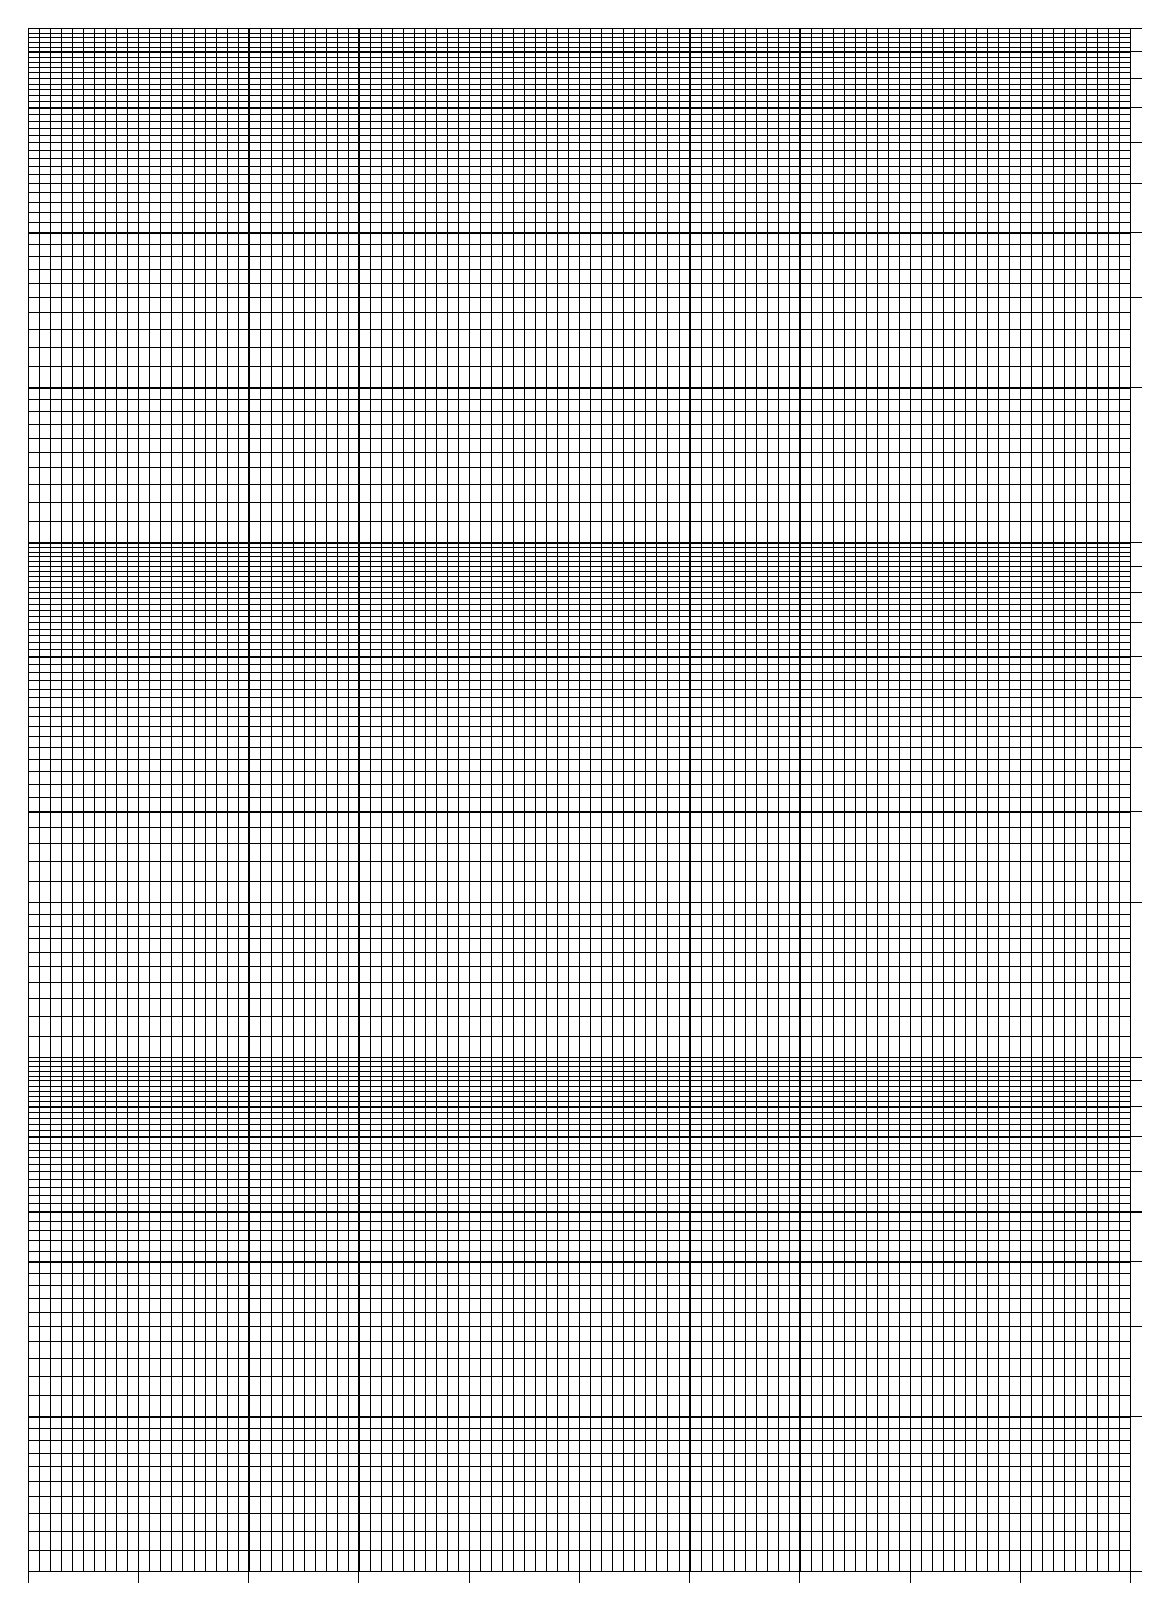
\begin{tikzpicture}[rotate=90,scale=1.4] %[xscale=1.3,yscale=1.3]
\draw[thin] (-0.1,0) --(14,0);

\foreach \x in {1,2,...,10} {
%\node at (7/ln 10 *ln \x, -0.5) {\pgfmathprintnumber[fixed,precision=1]{\x}}; 
\draw[thin] (14/3/ln 10 *ln \x,-0.1) -- ( 14/3/ln 10 *ln \x ,10);
}
\foreach \x in {1,1.1,...,2} {
\draw[ultra thin] (14/3/ln 10 *ln \x,0) -- ( 14/3/ln 10 *ln \x ,10);
}
\foreach \x in {2,2.2,...,10} {
\draw[ultra thin] (14/3/ln 10 *ln \x,0) -- ( 14/3/ln 10 *ln \x ,10);
}

\foreach \x in {1,2,...,10} {
\draw[thin] (14/3/ln 10 *ln \x+14/3,-0.1) -- ( 14/3/ln 10 *ln \x +14/3,10);
}
\foreach \x in {1,1.1,...,2} {
\draw[ultra thin] (14/3/ln 10 *ln \x+14/3,0) -- ( 14/3/ln 10 *ln \x+14/3 ,10);
}
\foreach \x in {2,2.2,...,10} {
\draw[ultra thin] (14/3/ln 10 *ln \x+14/3,0) -- ( 14/3/ln 10 *ln \x+14/3 ,10);
}

\foreach \x in {1,2,...,10} {
\draw[thin] (14/3/ln 10 *ln \x+14/3 +14/3,-0.1) -- ( 14/3/ln 10 *ln \x +14/3+14/3,10);
}
\foreach \x in {1,1.1,...,2} {
\draw[ultra thin] (14/3/ln 10 *ln \x+14/3+14/3,0) -- ( 14/3/ln 10 *ln \x +14/3+14/3,10);
}
\foreach \x in {2,2.2,...,10} {
\draw[ultra thin] (14/3/ln 10 *ln \x+14/3+14/3,0) -- ( 14/3/ln 10 *ln \x +14/3+14/3,10);
}


\foreach \x in {0.1,0.2,...,10} {
\draw[ultra thin] (0,\x) -- (14,\x);
}
\foreach \x in {1.0,2,...,10} {
\draw[thin] (-0.1,\x) -- (14,\x);
}
\end{tikzpicture}

%%%%%%%%%%%%%%%%%%%%%%%%%%%%%%%%%%%%%%%%%%%%%%%%%%%%%%%%%%%
%Linlog 3 decade END
%%%%%%%%%%%%%%%%%%%%%%%%%%%%%%%%%%%%%%%%%%%%%%%%%%%%%%%%%%




\chapter{Log-log 3 dekader}

%%%%%%%%%%%%%%%%%%%%%%%%%%%%%%%%%%%%%%%%%%%%%%%%%%%%%%%%%%%
%loglog 3 decade START
%%%%%%%%%%%%%%%%%%%%%%%%%%%%%%%%%%%%%%%%%%%%%%%%%%%%%%%%%%

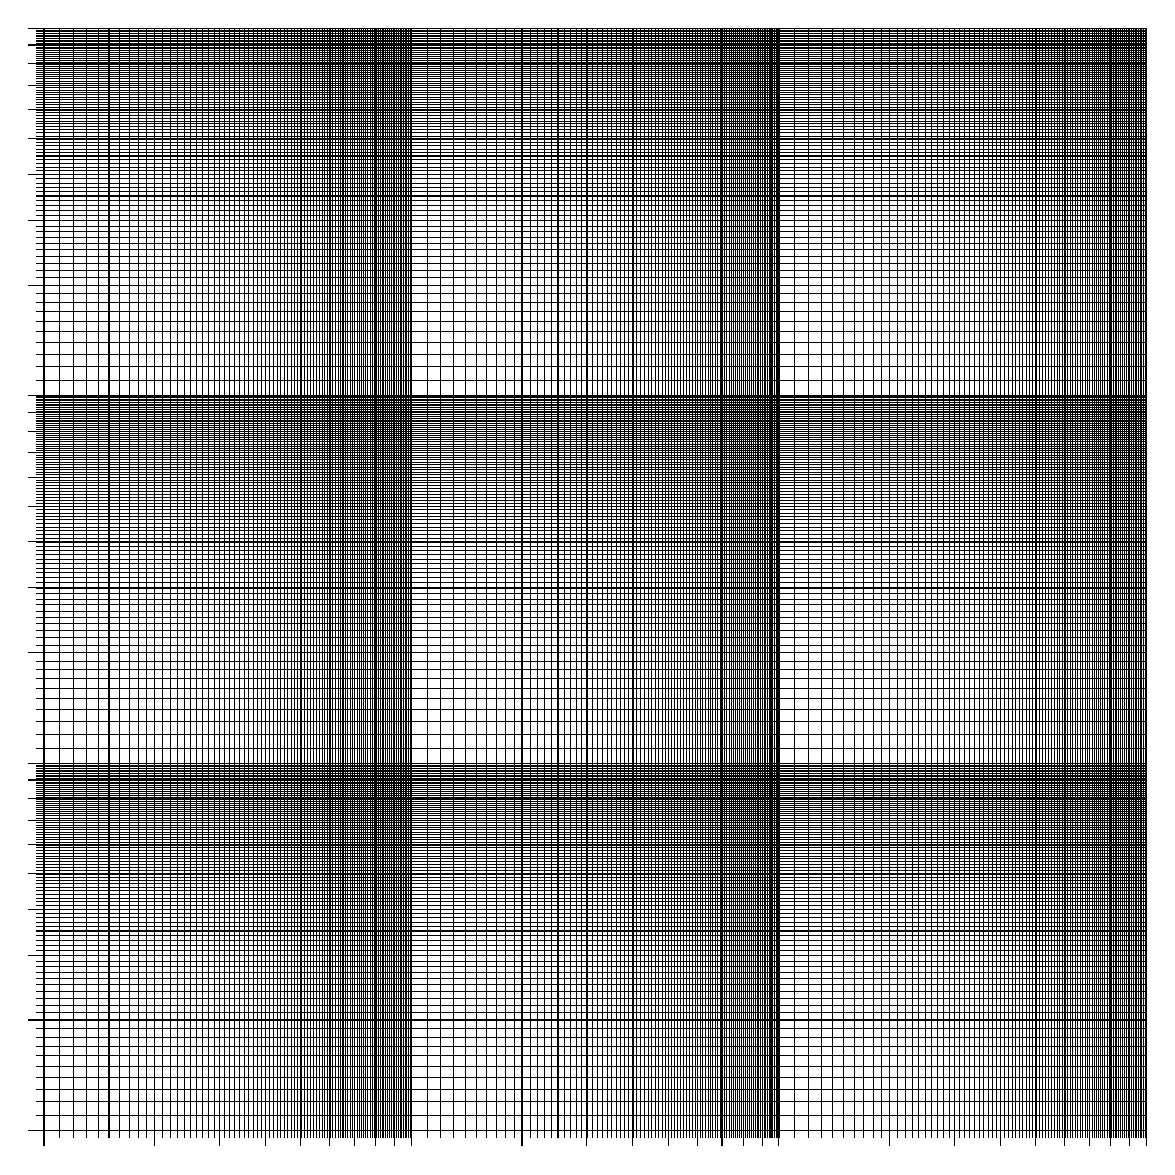
\begin{tikzpicture}[xscale=1,yscale=1] %[xscale=1.3,yscale=1.3]
\draw[ thin] (0,0) --(14,0);
% xaxis
% 1st decade
\foreach \x in {1,2,...,10} {
%\node at (14/2/ln 10 *ln \x, -0.5) {\pgfmathprintnumber[fixed,precision=1]{\x}}; 
\draw[thin] (14/3/ln 10 *ln \x,-0.2) -- ( 14/3/ln 10 *ln \x ,14);
}
\foreach \x in {1,1.5,...,10} {
\draw[very thin] (14/3/ln 10 *ln \x,-0.1) -- ( 14/3/ln 10 *ln \x ,14);
}
\foreach \x in {1.0,1.1,...,10} {
\draw[ultra thin] ( 14/3/ln 10 *ln \x, -0.1) -- ( 14/3/ln 10 *ln \x, 14);
}

% xaxis 
% 2nd decade
\foreach \x in {1,2,...,10} {
%\node at (14/2/ln 10 *ln \x+14/2, -0.5) {\pgfmathprintnumber[fixed,precision=1]{\x}}; 
\draw[thin] (14/3/ln 10 *ln \x+14/3,-0.2) -- ( 14/3/ln 10 *ln \x +14/3,14);
}
\foreach \x in {1,1.5,...,10} {
\draw[very thin] (14/3/ln 10 *ln \x+14/3,-0.1) -- ( 14/3/ln 10 *ln \x +14/3,14);
}
\foreach \x in {1.0,1.1,...,10} {
\draw[ultra thin] ( 14/3/ln 10 *ln \x+14/3, -0.1) -- ( 14/3/ln 10 *ln \x+14/3, 14);
}

% xaxis 
% 3rd decade
\foreach \x in {1,2,...,10} {
%\node at (14/2/ln 10 *ln \x+14/2, -0.5) {\pgfmathprintnumber[fixed,precision=1]{\x}}; 
\draw[thin] (14/3/ln 10 *ln \x+14/3+14/3,-0.2) -- ( 14/3/ln 10 *ln \x +14/3+14/3,14);
}
\foreach \x in {1,1.5,...,10} {
\draw[ very thin] (14/3/ln 10 *ln \x+14/3+14/3,-0.1) -- ( 14/3/ln 10 *ln \x +14/3+14/3,14);
}
\foreach \x in {1.0,1.1,...,10} {
\draw[ultra thin] ( 14/3/ln 10 *ln \x+14/3+14/3, -0.1) -- ( 14/3/ln 10 *ln \x+14/3+14/3, 14);
}

%\foreach \x in {1.0,1.1,...,10} {
%\draw[ultra thin] (14/ln 10 *ln \x,-0.1) -- ( 14/ln 10 *ln \x ,14);
%}
% yaxis
% 1st decade
\foreach \x in {1,2,...,10} {
%\node at (-0.4, 14/2/ln 10 *ln \x) {\tiny{\pgfmathprintnumber[fixed,precision=1]{\x}}}; 
\draw[thin] (-0.2 ,14/3/ln 10 *ln \x) -- ( 14 ,14/3/ln 10 *ln \x);
}
\foreach \x in {1,1.5,...,10} {
\draw[ very thin] (-0.1, 14/3/ln 10 *ln \x) -- ( 14, 14/3/ln 10 *ln \x);
}
\foreach \x in {1.0,1.1,...,10} {
\draw[ultra thin] (-0.1, 14/3/ln 10 *ln \x) -- ( 14, 14/3/ln 10 *ln \x);
}

% yaxis
% 2nd decade
\foreach \x in {2,3,...,10} {
%\node at (-0.4, 14/2/ln 10 *ln \x+14/2) {\tiny{\pgfmathprintnumber[fixed,precision=1]{\x}}}; 
\draw[thin] (-0.2 ,14/3/ln 10 *ln \x+14/3) -- ( 14 ,14/3/ln 10 *ln \x+14/3);
}
\foreach \x in {1,1.5,...,10} {
\draw[very thin] (-0.1, 14/3/ln 10 *ln \x+14/3) -- ( 14, 14/3/ln 10 *ln \x+14/3);
}
\foreach \x in {1.0,1.1,...,10} {
\draw[ultra thin] (-0.1, 14/3/ln 10 *ln \x+14/3) -- ( 14, 14/3/ln 10 *ln \x+14/3);
}
% yaxis
% 3rd decade
\foreach \x in {2,3,...,10} {
%\node at (-0.4, 14/3/ln 10 *ln \x+14/2) {\tiny{\pgfmathprintnumber[fixed,precision=1]{\x}}}; 
\draw[thin] (-0.2 ,14/3/ln 10 *ln \x+14/3+14/3) -- ( 14 ,14/3/ln 10 *ln \x+14/3+14/3);
}
\foreach \x in {1,1.5,...,10} {
\draw[very thin] (-0.1, 14/3/ln 10 *ln \x+14/3+14/3) -- ( 14, 14/3/ln 10 *ln \x+14/3+14/3);
}
\foreach \x in {1.0,1.1,...,10} {
\draw[ultra thin] (-0.1, 14/3/ln 10 *ln \x+14/3+14/3) -- ( 14, 14/3/ln 10 *ln \x+14/3+14/3);
}


\end{tikzpicture}
%%%%%%%%%%%%%%%%%%%%%%%%%%%%%%%%%%%%%%%%%%%%%%%%%%%%%%%%%%%
%loglog 3 decade END
%%%%%%%%%%%%%%%%%%%%%%%%%%%%%%%%%%%%%%%%%%%%%%%%%%%%%%%%%%




\end{document}